\documentclass[12pt]{article}

% ── Packages ──────────────────────────────────────────────────────────────
\usepackage[margin=1in]{geometry}
\usepackage{amsmath, amssymb}
\usepackage{graphicx}
\usepackage{booktabs}
\usepackage{hyperref}
\usepackage{natbib}
\usepackage{caption}
\usepackage{xcolor}
\usepackage{float}
\usepackage{multirow}

% ── Title ─────────────────────────────────────────────────────────────────
\title{\textbf{Signal Peptide Efficiency Prediction Using Protein Language Model Embeddings and Neural Network Regression}}

\author{
  Mehak Wadhwa \\
  Department of Chemistry, Fordham University \\
  Advisor: Dr.\ Joshua Schrier
}

\date{\today}

\begin{document}
\maketitle

% ══════════════════════════════════════════════════════════════════════════
\begin{abstract}
Signal peptides direct protein secretion in bacteria and are critical targets for optimizing recombinant protein production.
We present a systematic comparison of machine learning approaches for predicting signal peptide efficiency in \textit{Bacillus subtilis}, evaluating random forest (RF) and neural network (NN) regressors across four feature representations: 156 physicochemical descriptors and three protein language model (PLM) embedding sets (ESM2-650M, ESM2-3B, Ginkgo-AA0).
A vector regression approach, predicting 10-bin probability distributions via a softmax output with focal loss \citep{lin2017focal}, achieves a test MSE of 1.001 with Ginkgo-AA0 embeddings using an 80/20 validation split.
Further optimization using full-data training with increased dropout and a deeper architecture yields a 5-seed ensemble MSE of 0.932 [0.823, 1.054] (95\% bootstrap CI), surpassing both the physicochemical baseline of 1.22 \citep{grasso2023} and a prior benchmark of 0.953 (J.\ Schrier, personal communication).
Cross-dataset evaluation on four external signal peptide datasets reveals significant negative zero-shot Spearman correlations; fine-tuning the output head on target-domain data reverses these for two of four datasets, demonstrating partial transferability of learned representations.
Applied to 4832 designed signal peptide variants using both physicochemical features and ESM2-650M embeddings, RF and NN models achieve Spearman $\rho = 0.36$--0.39 and classification accuracy of 72--74\% for ranking variants relative to wild type, with the ESM2-650M NN achieving the highest rank correlation ($\rho = 0.394$), demonstrating practical utility for guiding experimental prioritization.
\end{abstract}

% ══════════════════════════════════════════════════════════════════════════
\section{Introduction}
\label{sec:intro}

Signal peptides are short N-terminal sequences (typically 15--30 amino acids) that direct nascent proteins through cellular secretion machinery.
In industrial biotechnology, the choice of signal peptide can determine whether a recombinant protein is produced at commercially viable yields or fails entirely \citep{grasso2023}.
For organisms like \textit{Bacillus subtilis}, a workhorse of industrial enzyme production, optimizing signal peptide selection is essential for maximizing secretion efficiency.

Traditional approaches to signal peptide optimization rely on experimental screening, which is time-consuming and expensive.
Machine learning offers the potential to predict secretion efficiency from sequence alone, enabling rational design of signal peptide--protein combinations.
\citet{grasso2023} constructed a library of signal peptide variants and trained a random forest regressor on 156 physicochemical descriptors, achieving a test MSE of 1.22 for predicting whole-cell activity (WA).

Recent advances in protein language models (PLMs) provide an alternative to hand-crafted features.
Models like ESM-2 \citep{lin2023} learn rich representations of protein sequences from evolutionary data, capturing structural and functional information that may not be encoded in traditional descriptors.
However, effectively leveraging these high-dimensional embeddings (1280--2560 dimensions) requires appropriate model architectures and hyperparameter tuning.

In this work, we systematically evaluate signal peptide efficiency prediction across multiple feature representations and model types.
We identified several methodological considerations in applying machine learning to this problem:
\begin{enumerate}
    \item Ensuring reproducibility through direct loading from source data files
    \item Performing hyperparameter search independently for each feature type
    \item Using regression (not classification) for continuous efficiency prediction
    \item Scaling neural network architectures to input dimensionality
\end{enumerate}

Our analysis reveals a clear interaction between model type and feature representation: neural networks substantially outperform random forests when given PLM embeddings, but underperform on physicochemical features.
Beyond this core comparison, we extend the analysis in four directions: (i) a vector regression approach that predicts bin probability distributions instead of scalar WA, yielding further performance gains; (ii) full-data architecture and regularization optimization that pushes vector regression below the prior state of the art; (iii) cross-dataset generalization evaluation against four external datasets; and (iv) a design task evaluating model utility for ranking novel signal peptide variants.

% ══════════════════════════════════════════════════════════════════════════
\section{Methods}
\label{sec:methods}

\subsection{Data}
\label{sec:data}

All data originate from the supplementary material of \citet{grasso2023}.
The dataset comprises signal peptide variants fused to a $\beta$-glucuronidase reporter in \textit{B.\ subtilis}, with whole-cell activity (WA) measured as a proxy for secretion efficiency.
Quality filters follow the original protocol: signal peptide length 10--40 amino acids, WA values between 1.0 and 10.0.
The original train/test partition is preserved, yielding 3085 training and 1323 test samples for physicochemical features.

We evaluate four feature representations:
\begin{itemize}
    \item \textbf{PhysChem}: 156 physicochemical descriptors from \citet{grasso2023}, including amino acid composition, hydrophobicity, and secondary structure propensities for each signal peptide region.
    \item \textbf{ESM2-650M}: 1280-dimensional mean-pooled embeddings from the 650M-parameter ESM-2 model \citep{lin2023}.
    \item \textbf{ESM2-3B}: 2560-dimensional embeddings from the 3B-parameter ESM-2 model.
    \item \textbf{Ginkgo-AA0}: 1280-dimensional embeddings from Ginkgo Bioworks' AA0 protein language model \citep{ginkgo2024}, trained on proprietary protein sequence data.
\end{itemize}

The PLM datasets contain 3095 training and 1326 test samples (minor differences arise from sequence-level filtering).

\subsection{Preprocessing}
\label{sec:preprocessing}

Features are standardized to zero mean and unit variance using statistics computed on training data only.
Target skewness is evaluated; log$_{1+x}$ transformation is applied when $|\text{skew}| > 1.0$.
For all datasets in this study, skewness was 0.116, so no transformation was applied.

\subsection{Random Forest Models}
\label{sec:rf}

We first reproduce the baseline result using the exact hyperparameters from \citet{grasso2023}: 75 trees, max depth 25, \texttt{min\_samples\_split} = 0.001, \texttt{min\_samples\_leaf} = 0.0001, with all features available at each split.

For systematic comparison, we perform randomized hyperparameter search independently for each feature type using 100 configurations evaluated under 5-fold cross-validation.
The search space includes: number of trees $\in \{50, 75, 100, 150, 200, 300\}$, max depth $\in \{10, 15, 20, 25, 30, \text{None}\}$, minimum samples for splitting $\in \{2, 5, 10, 0.001, 0.01\}$, minimum samples per leaf $\in \{1, 2, 4, 0.0001, 0.001\}$, and fraction of features per split $\in \{\text{sqrt}, \text{log2}, 0.5, 0.75, 1.0\}$.

\subsection{Neural Network Regression}
\label{sec:nn}

We train feedforward neural networks with the following architecture for each hidden layer: fully connected $\rightarrow$ batch normalization $\rightarrow$ ReLU activation $\rightarrow$ dropout.
The output layer is a single neuron with linear activation, trained to minimize MSE.

Hidden layer sizes are scaled to input dimensionality:
\begin{itemize}
    \item PhysChem (156d): architectures from $\{[128], [128, 64], [256, 128]\}$
    \item ESM2-650M / Ginkgo-AA0 (1280d): $\{[256], [512, 256], [256, 128]\}$
    \item ESM2-3B (2560d): $\{[512], [512, 256], [1024, 512]\}$
\end{itemize}

Additional hyperparameters: dropout rate $\in \{0.2, 0.3, 0.4, 0.5\}$, L2 regularization $\in \{10^{-4}, 10^{-3}, 10^{-2}\}$, learning rate $\in \{10^{-3}, 5\times10^{-4}, 10^{-4}\}$, and batch size $\in \{32, 64\}$.
We sample 40 configurations per feature type, training each with the Adam optimizer for up to 200 epochs with early stopping (patience 15) and learning rate reduction on plateau.
An 80/20 train/validation split is used for model selection; the configuration with the lowest validation MSE is evaluated on the held-out test set.

\subsection{Multi-Seed Ensemble Protocol}
\label{sec:ensemble}

To reduce variance from random initialization and data splitting, we employ a 5-seed ensemble protocol with seeds $\{42, 123, 456, 789, 1024\}$.
For each seed, the training set is split 80/20 into training and validation subsets; a model is trained with early stopping on the validation loss.
The ensemble prediction is the arithmetic mean of the five per-seed predictions.
This protocol is used for the neural network models in Sections~\ref{sec:vector}--\ref{sec:cross_dataset_methods}.

\subsection{Vector Regression}
\label{sec:vector}

Rather than predicting a scalar WA value, we predict the 10-dimensional bin probability distribution from which WA is derived.
The WA measurement in \citet{grasso2023} is computed from fluorescence-activated cell sorting into 10 bins, with $\text{WA} = \sum_{i=1}^{10} i \cdot p_i$ where $p_i$ is the fraction of cells in bin $i$.
Some sequences exhibit bimodal bin distributions where the WA falls between two peaks (Figure~\ref{fig:bimodal}), illustrating that the scalar WA can be a poor summary of the underlying data; predicting the full distribution preserves this information.

\begin{figure}[H]
    \centering
    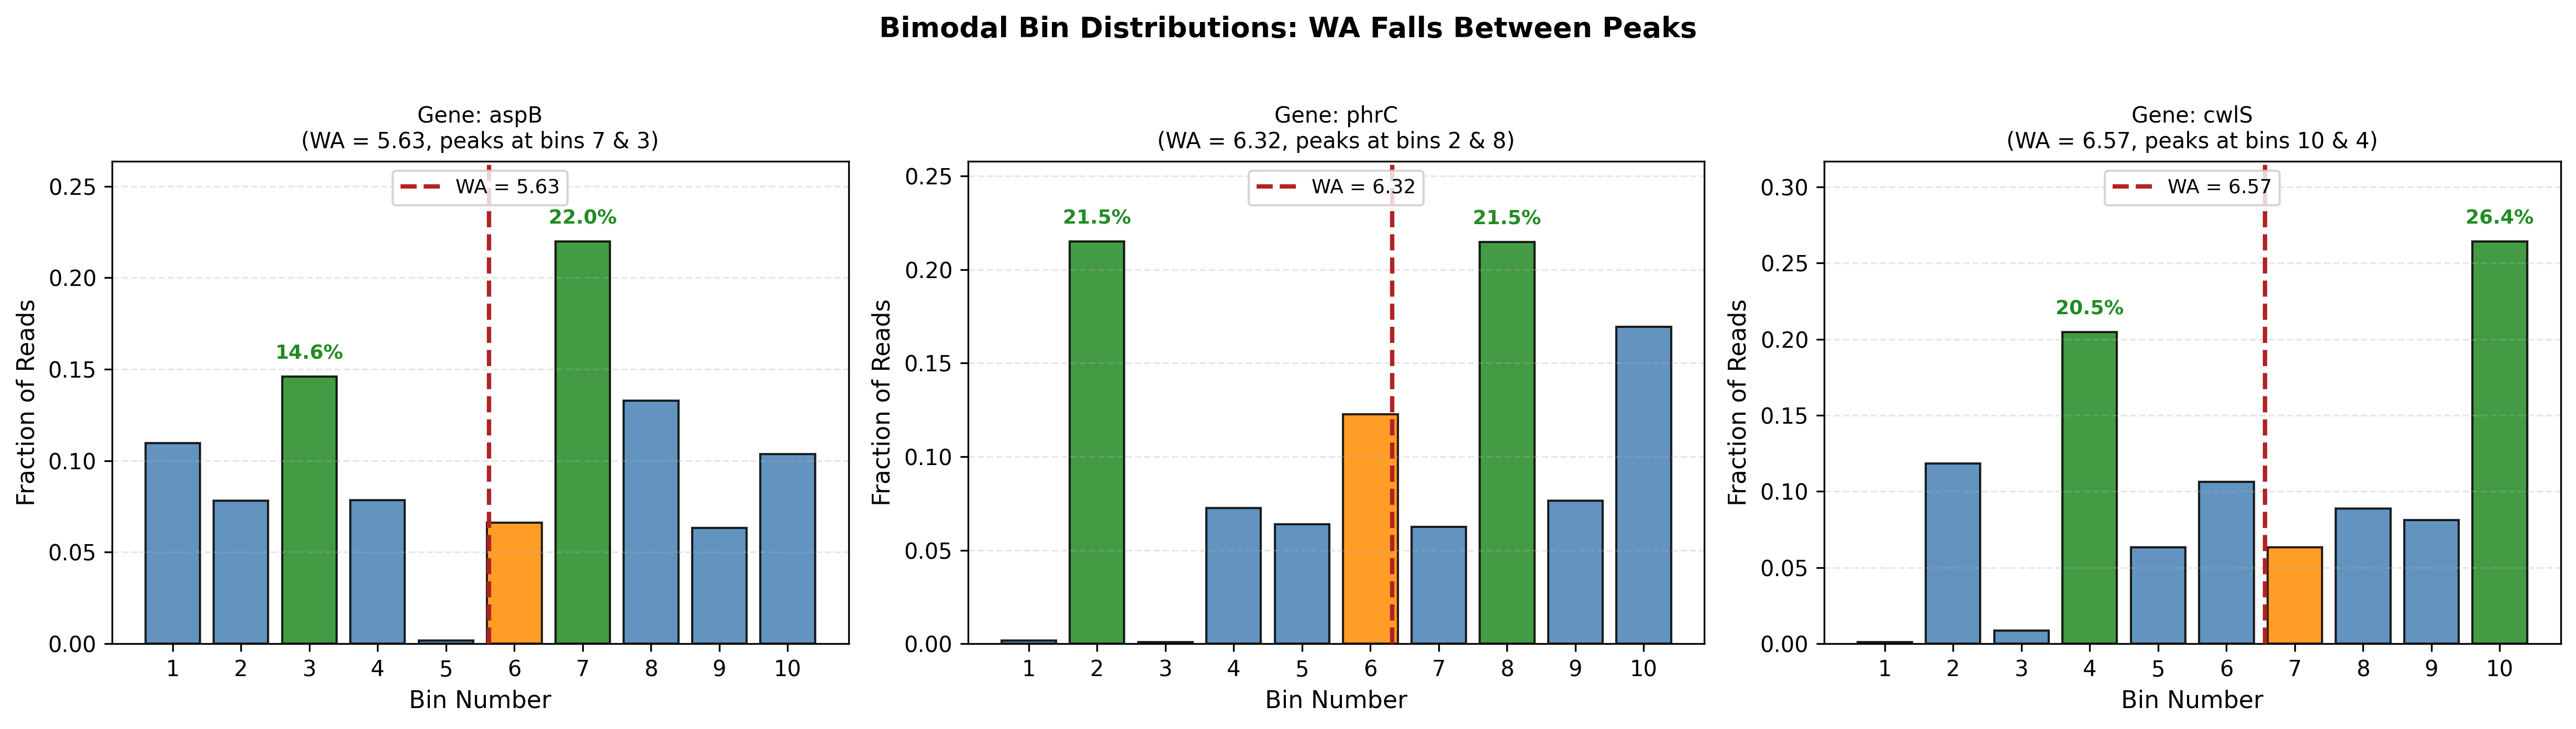
\includegraphics[width=0.95\textwidth]{../figures/bimodal_bin_distributions.png}
    \caption{Examples of bimodal experimental bin probability distributions from the Grasso dataset, selected as variants with probability mass spread across many bins and two distinct peaks. Left: gene \textit{aspB}, variant MKLAKRVSALTPSTTLAITQKAKEL (row 8123, WA = 5.63, peaks at bins 3 and 7). Center: gene \textit{phrC}, variant MKLKSKLFVICLAAAAIFRKKKVSANAEALDF (row 3419, WA = 6.32, peaks at bins 2 and 8). Right: gene \textit{cwlS}, variant MSSGIIVAGLAVSAVVGSSMAAAPAEAKTI (row 9974, WA = 6.57, peaks at bins 4 and 10). The red dashed line indicates the WA, which falls in a valley between the two peaks in each case, demonstrating that the scalar WA can be a poor summary of the underlying distribution.}
    \label{fig:bimodal}
\end{figure}

The vector regression architecture uses two hidden layers of 256 units each with LeakyReLU activation and 20\% dropout, followed by a 10-unit output layer with softmax activation to produce a valid probability distribution.
Unlike the scalar NN (Section~\ref{sec:nn}), batch normalization is omitted.
Two loss functions are compared: categorical cross-entropy and focal loss \citep{lin2017focal}, defined as $\text{FL}(p_t) = -\alpha(1-p_t)^\gamma \log(p_t)$ with $\alpha = 0.25$ and $\gamma = 2.0$.
Focal loss down-weights well-classified examples, encouraging the model to focus on samples with ambiguous bin distributions.
Each embedding--loss combination is trained as a 5-seed ensemble (Section~\ref{sec:ensemble}).
After prediction, WA is recovered as $\hat{\text{WA}} = \hat{\mathbf{p}} \cdot [1, 2, \ldots, 10]^\top$.

Rows with missing bin probabilities (27 training, 53 test) are excluded from vector regression training, yielding 3068 training samples.
The validation-split models (Section~\ref{sec:vector_results}) evaluate on the 1273 test samples with complete bin data; the optimized models described below evaluate on all 1326 test samples using WA as the target.

\label{sec:fulldata}
\paragraph{Architecture and regularization optimization.}
Because the base vector model (MSE 1.001) still falls short of the 0.953 benchmark obtained by Schrier using a similar architecture, we explore whether removing the validation split and compensating with explicit regularization can close this gap.
Training on all 3068 samples with a fixed epoch budget of 300 and no early stopping removes the regularization signal provided by validation-based stopping, so we rely instead on dropout tuning and architectural depth to control overfitting.
We explore:
\begin{itemize}
    \item \textbf{Dropout rate}: 0.15, 0.20, 0.25, 0.30, and 0.35 (vs.\ the base 0.20), applied to a deeper (256, 256, 128) three-layer architecture with 5-seed ensembles.
    \item \textbf{Deeper architectures}: 4-layer configurations including (256, 256, 128, 64), (384, 384, 256, 128), and others, with 5-seed ensembles.
    \item \textbf{Cosine annealing}: Learning rate schedule $\eta_t = \eta_0 \cdot \frac{1}{2}(1 + \cos(\pi t / T))$ combined with deeper architectures.
    \item \textbf{Large ensembles}: 20-seed ensembles with the best configurations.
    \item \textbf{Mixed-architecture ensemble}: Averaging predictions from multiple distinct architectures.
\end{itemize}
All configurations use Ginkgo-AA0 embeddings and focal loss.
Each 5-seed ensemble uses seeds $\{42, 123, 456, 789, 1024\}$ with independent random initialization; predictions are averaged across seeds.

\subsection{Cross-Dataset Generalization}
\label{sec:cross_dataset_methods}

The results above demonstrate strong predictive performance within the Grasso dataset, but a model's practical value depends on whether it transfers to new experimental contexts.
To evaluate this, we test the best ESM2-650M RF and the 5-seed NN ensemble on four external datasets:
\begin{itemize}
    \item \textbf{Wu} \citep{wu2020}: 81 signal peptides in \textit{E.\ coli} with binary secretion labels.
    \item \textbf{Xue} \citep{xue2023}: 322 signal peptides in \textit{S.\ cerevisiae} with enzyme activity measurements.
    \item \textbf{Zhang-P43 / Zhang-PglVM} \citep{zhang2016}: 114 signal peptides in \textit{B.\ subtilis} measured under two different promoters.
\end{itemize}
Spearman rank correlation serves as the primary metric, as it is invariant to differences in scale and units between datasets.
For the Zhang datasets, we additionally evaluate cross-promoter prediction consistency: whether the model predicts the same relative ranking for the same signal peptides under two promoters.

\paragraph{Transfer learning via fine-tuning.}
To test whether the negative zero-shot correlations can be reversed with limited target-domain data,
we fine-tune a vector regression ensemble with the same optimized architecture
(focal loss, (256, 256, 128), dropout 0.35) but trained on ESM2-650M embeddings,
since Ginkgo-AA0 embeddings are not available for external sequences.
Fine-tuning uses 5-fold cross-validation with 5 random seeds per fold.
The pretrained model's first two hidden blocks (6 layers) are frozen, and the 10-unit softmax
output head is replaced with a task-specific head: a single sigmoid unit for the binary Wu dataset,
or a single linear unit for the continuous datasets (Xue, Zhang-P43, Zhang-PglVM).
Fine-tuning uses a reduced learning rate ($10^{-4}$, 5$\times$ lower than pretraining),
batch size 32, up to 100 epochs with early stopping (patience 10), and MSE loss
(binary cross-entropy for Wu). Spearman $\rho$ is averaged across folds.

\subsection{Design Task Evaluation}
\label{sec:design_methods}

The Grasso library contains 4836 designed signal peptide variants with known WA values (Set = NaN in the original data, after excluding 393 that overlap with the train/test sets), spanning 134 genes.
A minimum of 5 variants per gene is required for per-gene metrics, yielding 4832 variants across 131 genes for evaluation.
We evaluate two feature representations: the 156 physicochemical features available from the source data, and ESM2-650M embeddings (1280 dimensions) generated via mean-pooled representations from the pretrained model \citep{lin2023}.
For each feature type, RF and NN models are trained on the Grasso training set with the best hyperparameters from Sections~\ref{sec:rf}--\ref{sec:nn} and evaluated on the design variants.
Wild-type WA for each gene is determined by matching the wild-type signal peptide sequence (from the ``WT sequences'' sheet of the source spreadsheet) against Library rows with the same amino acid sequence and taking the mean WA of matching rows, yielding WT WA values for 137 genes.
Per-gene and overall Spearman $\rho$ are computed, along with classification accuracy for predicting whether a variant performs better or worse than wild type.

\subsection{Evaluation}
\label{sec:metrics}

All models are evaluated on the same held-out test set using mean squared error (MSE), coefficient of determination ($R^2$), and Spearman rank correlation ($\rho$).
MSE is the primary metric for consistency with prior work.

% ══════════════════════════════════════════════════════════════════════════
\section{Results}
\label{sec:results}

\subsection{Baseline Reproduction}

Using the exact parameters from \citet{grasso2023}, we obtain a test MSE of 1.193 ($R^2 = 0.750$, Spearman $\rho = 0.859$), within 2.2\% of the reported value of 1.22.
Figure~\ref{fig:grasso_repro} shows predicted versus actual WA values.

\begin{figure}[H]
    \centering
    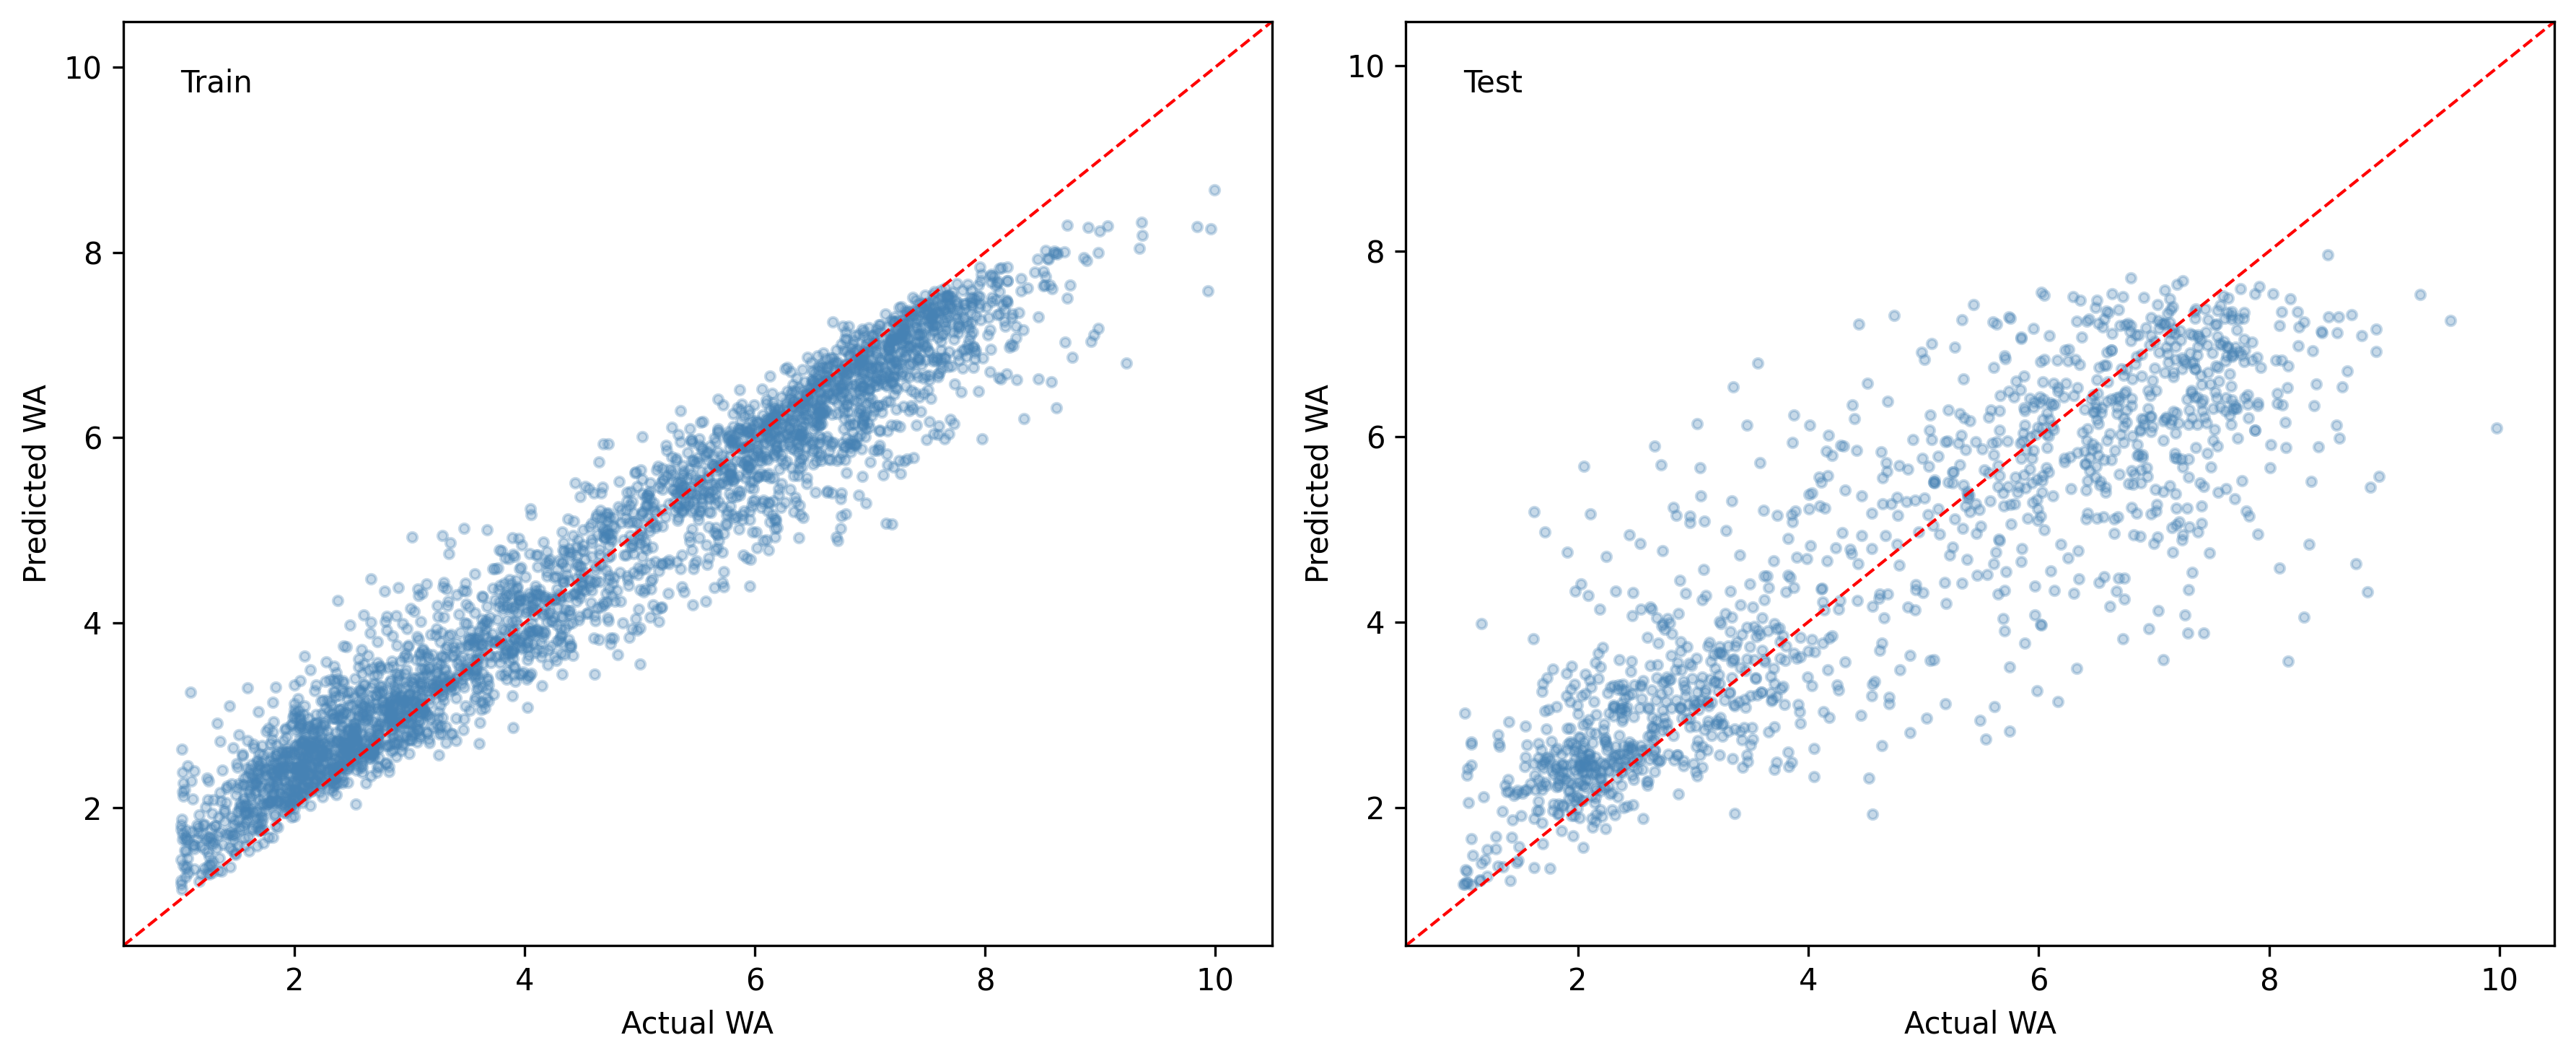
\includegraphics[width=0.95\textwidth]{../figures/grasso_reproduction.png}
    \caption{Baseline reproduction using physicochemical features and the exact random forest parameters from \citet{grasso2023}. Predicted vs.\ actual whole-cell activity for training (left) and test (right) sets. Dashed line indicates perfect prediction.}
    \label{fig:grasso_repro}
\end{figure}

\subsection{Scalar Model Comparison}

With the baseline established, we compare all model--feature combinations.
Table~\ref{tab:comparison} presents results for all scalar model--feature combinations.

\begin{table}[H]
\centering
\caption{Test set performance across all scalar model and feature type combinations, sorted by MSE. The $\Delta$ column shows percent change relative to the \citet{grasso2023} baseline MSE of 1.22.}
\label{tab:comparison}
\begin{tabular}{llcccc}
\toprule
Feature Type & Model & Test MSE & Test $R^2$ & Spearman $\rho$ & $\Delta$ \\
\midrule
Ginkgo-AA0 & NN & \textbf{1.050} & \textbf{0.780} & \textbf{0.866} & $-$14.0\% \\
ESM2-3B & NN & 1.067 & 0.776 & 0.861 & $-$12.5\% \\
ESM2-650M & NN & 1.090 & 0.771 & 0.861 & $-$10.6\% \\
Ginkgo-AA0 & RF & 1.158 & 0.757 & 0.857 & $-$5.1\% \\
ESM2-650M & RF & 1.189 & 0.750 & 0.853 & $-$2.5\% \\
PhysChem & RF (baseline) & 1.193 & 0.750 & 0.859 & $-$2.2\% \\
PhysChem & RF (tuned) & 1.208 & 0.747 & 0.857 & $-$1.0\% \\
ESM2-3B & RF & 1.245 & 0.739 & 0.849 & $+$2.0\% \\
PhysChem & NN & 1.328 & 0.721 & 0.840 & $+$8.8\% \\
\bottomrule
\end{tabular}
\end{table}

Figure~\ref{fig:comparison} visualizes these results as a grouped bar chart.

\begin{figure}[H]
    \centering
    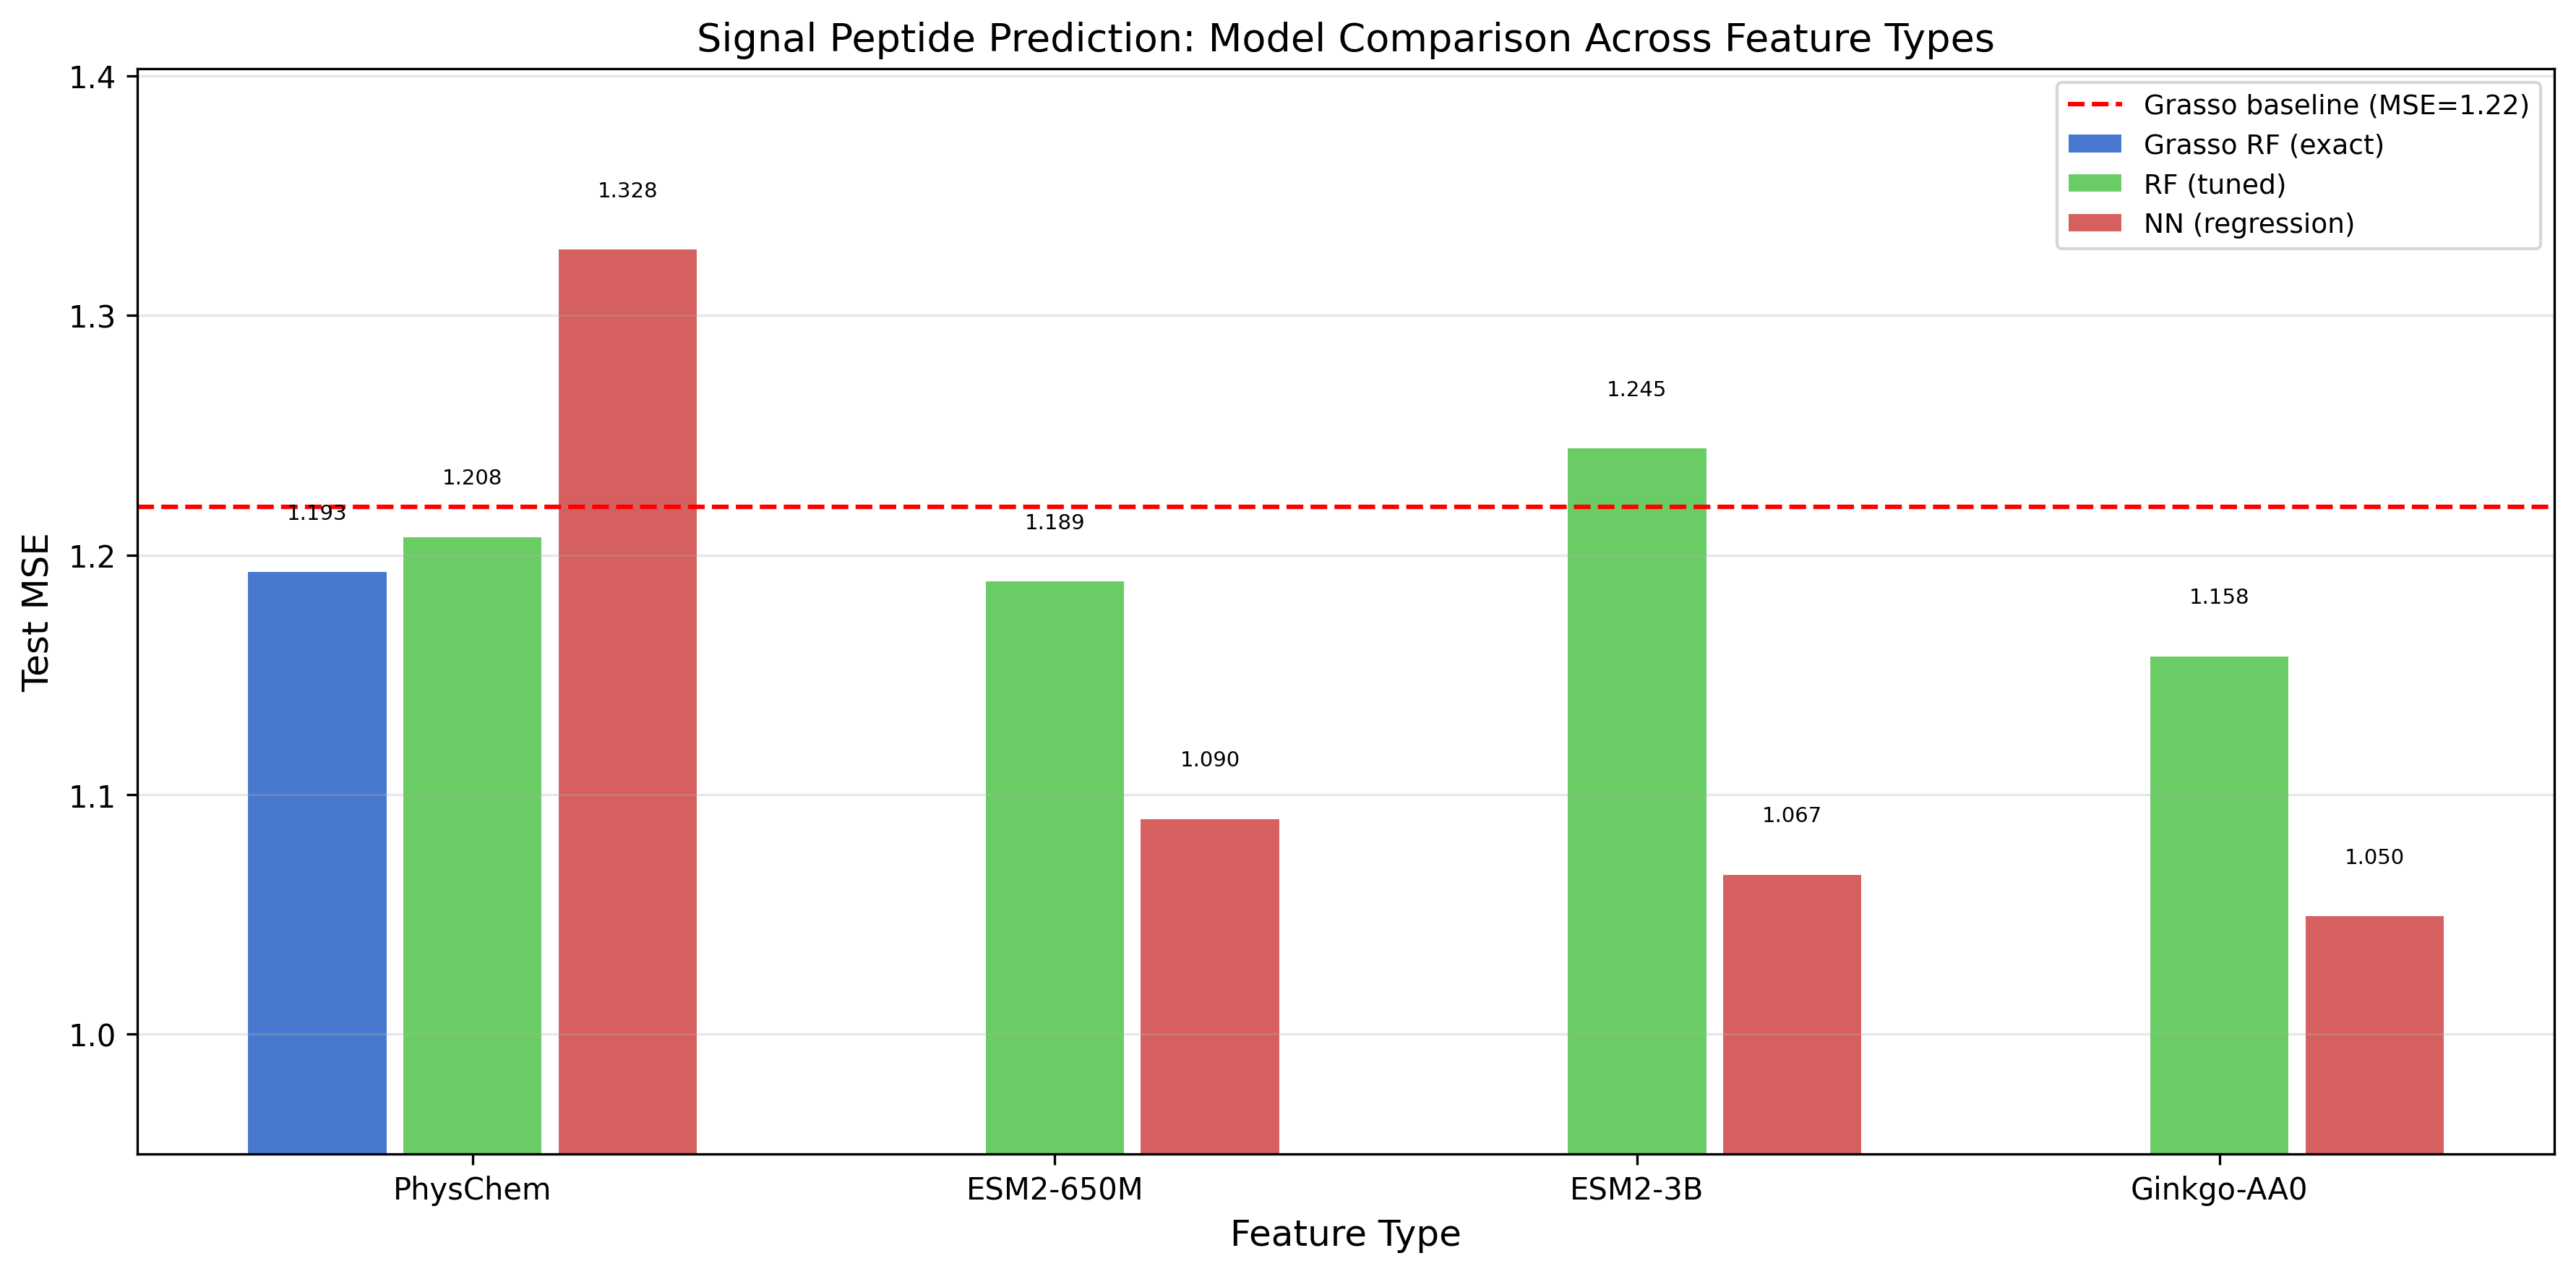
\includegraphics[width=0.95\textwidth]{../figures/final_comparison.png}
    \caption{Test MSE across feature types and model architectures. Dashed red line indicates the baseline MSE of 1.22. Lower values indicate better performance.}
    \label{fig:comparison}
\end{figure}

\paragraph{Random Forest Results.}
Tuned RF models achieve MSE values between 1.16 and 1.25 across all feature types.
Ginkgo-AA0 embeddings yield the best RF result (MSE 1.158), followed by ESM2-650M (1.189) and physicochemical features (1.208).
ESM2-3B performs worst (MSE 1.245), likely due to the curse of dimensionality in tree-based splitting with 2560 features.

\paragraph{Neural Network Results.}
The ranking changes substantially for neural networks.
All three PLM embedding types outperform the baseline, with Ginkgo-AA0 achieving the best scalar result (MSE 1.050, $R^2 = 0.780$).
However, the NN trained on physicochemical features performs worse than the RF baseline (MSE 1.328 vs.\ 1.193).

\subsection{Vector Regression}
\label{sec:vector_results}

Given that neural networks with PLM embeddings outperform all other scalar approaches, we next ask whether predicting the full bin probability distribution can yield further gains.
Table~\ref{tab:vector} presents results for vector regression models.

\begin{table}[H]
\centering
\caption{Vector regression test set performance (5-seed ensembles, $N_{\text{test}} = 1273$). WA is recovered from predicted bin probabilities. See text for caveats on comparing with Table~\ref{tab:comparison}.}
\label{tab:vector}
\begin{tabular}{llccc}
\toprule
Embedding & Loss & Test MSE & Test $R^2$ & Spearman $\rho$ \\
\midrule
Ginkgo-AA0 & Focal & \textbf{1.001} & \textbf{0.790} & \textbf{0.867} \\
Ginkgo-AA0 & Cross-entropy & 1.003 & 0.790 & 0.867 \\
ESM2-650M & Focal & 1.049 & 0.780 & 0.859 \\
ESM2-650M & Cross-entropy & 1.054 & 0.779 & 0.861 \\
ESM2-3B & Cross-entropy & 1.109 & 0.767 & 0.857 \\
ESM2-3B & Focal & 1.117 & 0.766 & 0.856 \\
\bottomrule
\end{tabular}
\end{table}

The best vector regression model (Ginkgo-AA0 + focal loss) achieves MSE = 1.001, a 4.7\% improvement over the best scalar NN (1.050) and an 18\% improvement over the baseline (1.22).
Focal loss provides a marginal edge over cross-entropy for Ginkgo-AA0 and ESM2-650M, though the differences are small.
ESM2-3B again performs worst among the three PLMs, consistent with the scalar regression results.
Note that the vector regression test set (1273 samples) is smaller than the scalar test set (1326 samples) due to exclusion of rows with missing bin probabilities, and the vector results use 5-seed ensembles rather than single configurations, so direct MSE comparison between Tables~\ref{tab:comparison} and \ref{tab:vector} should be interpreted with caution.
Figure~\ref{fig:vector} shows the comparison across embeddings and loss functions.

\begin{figure}[H]
    \centering
    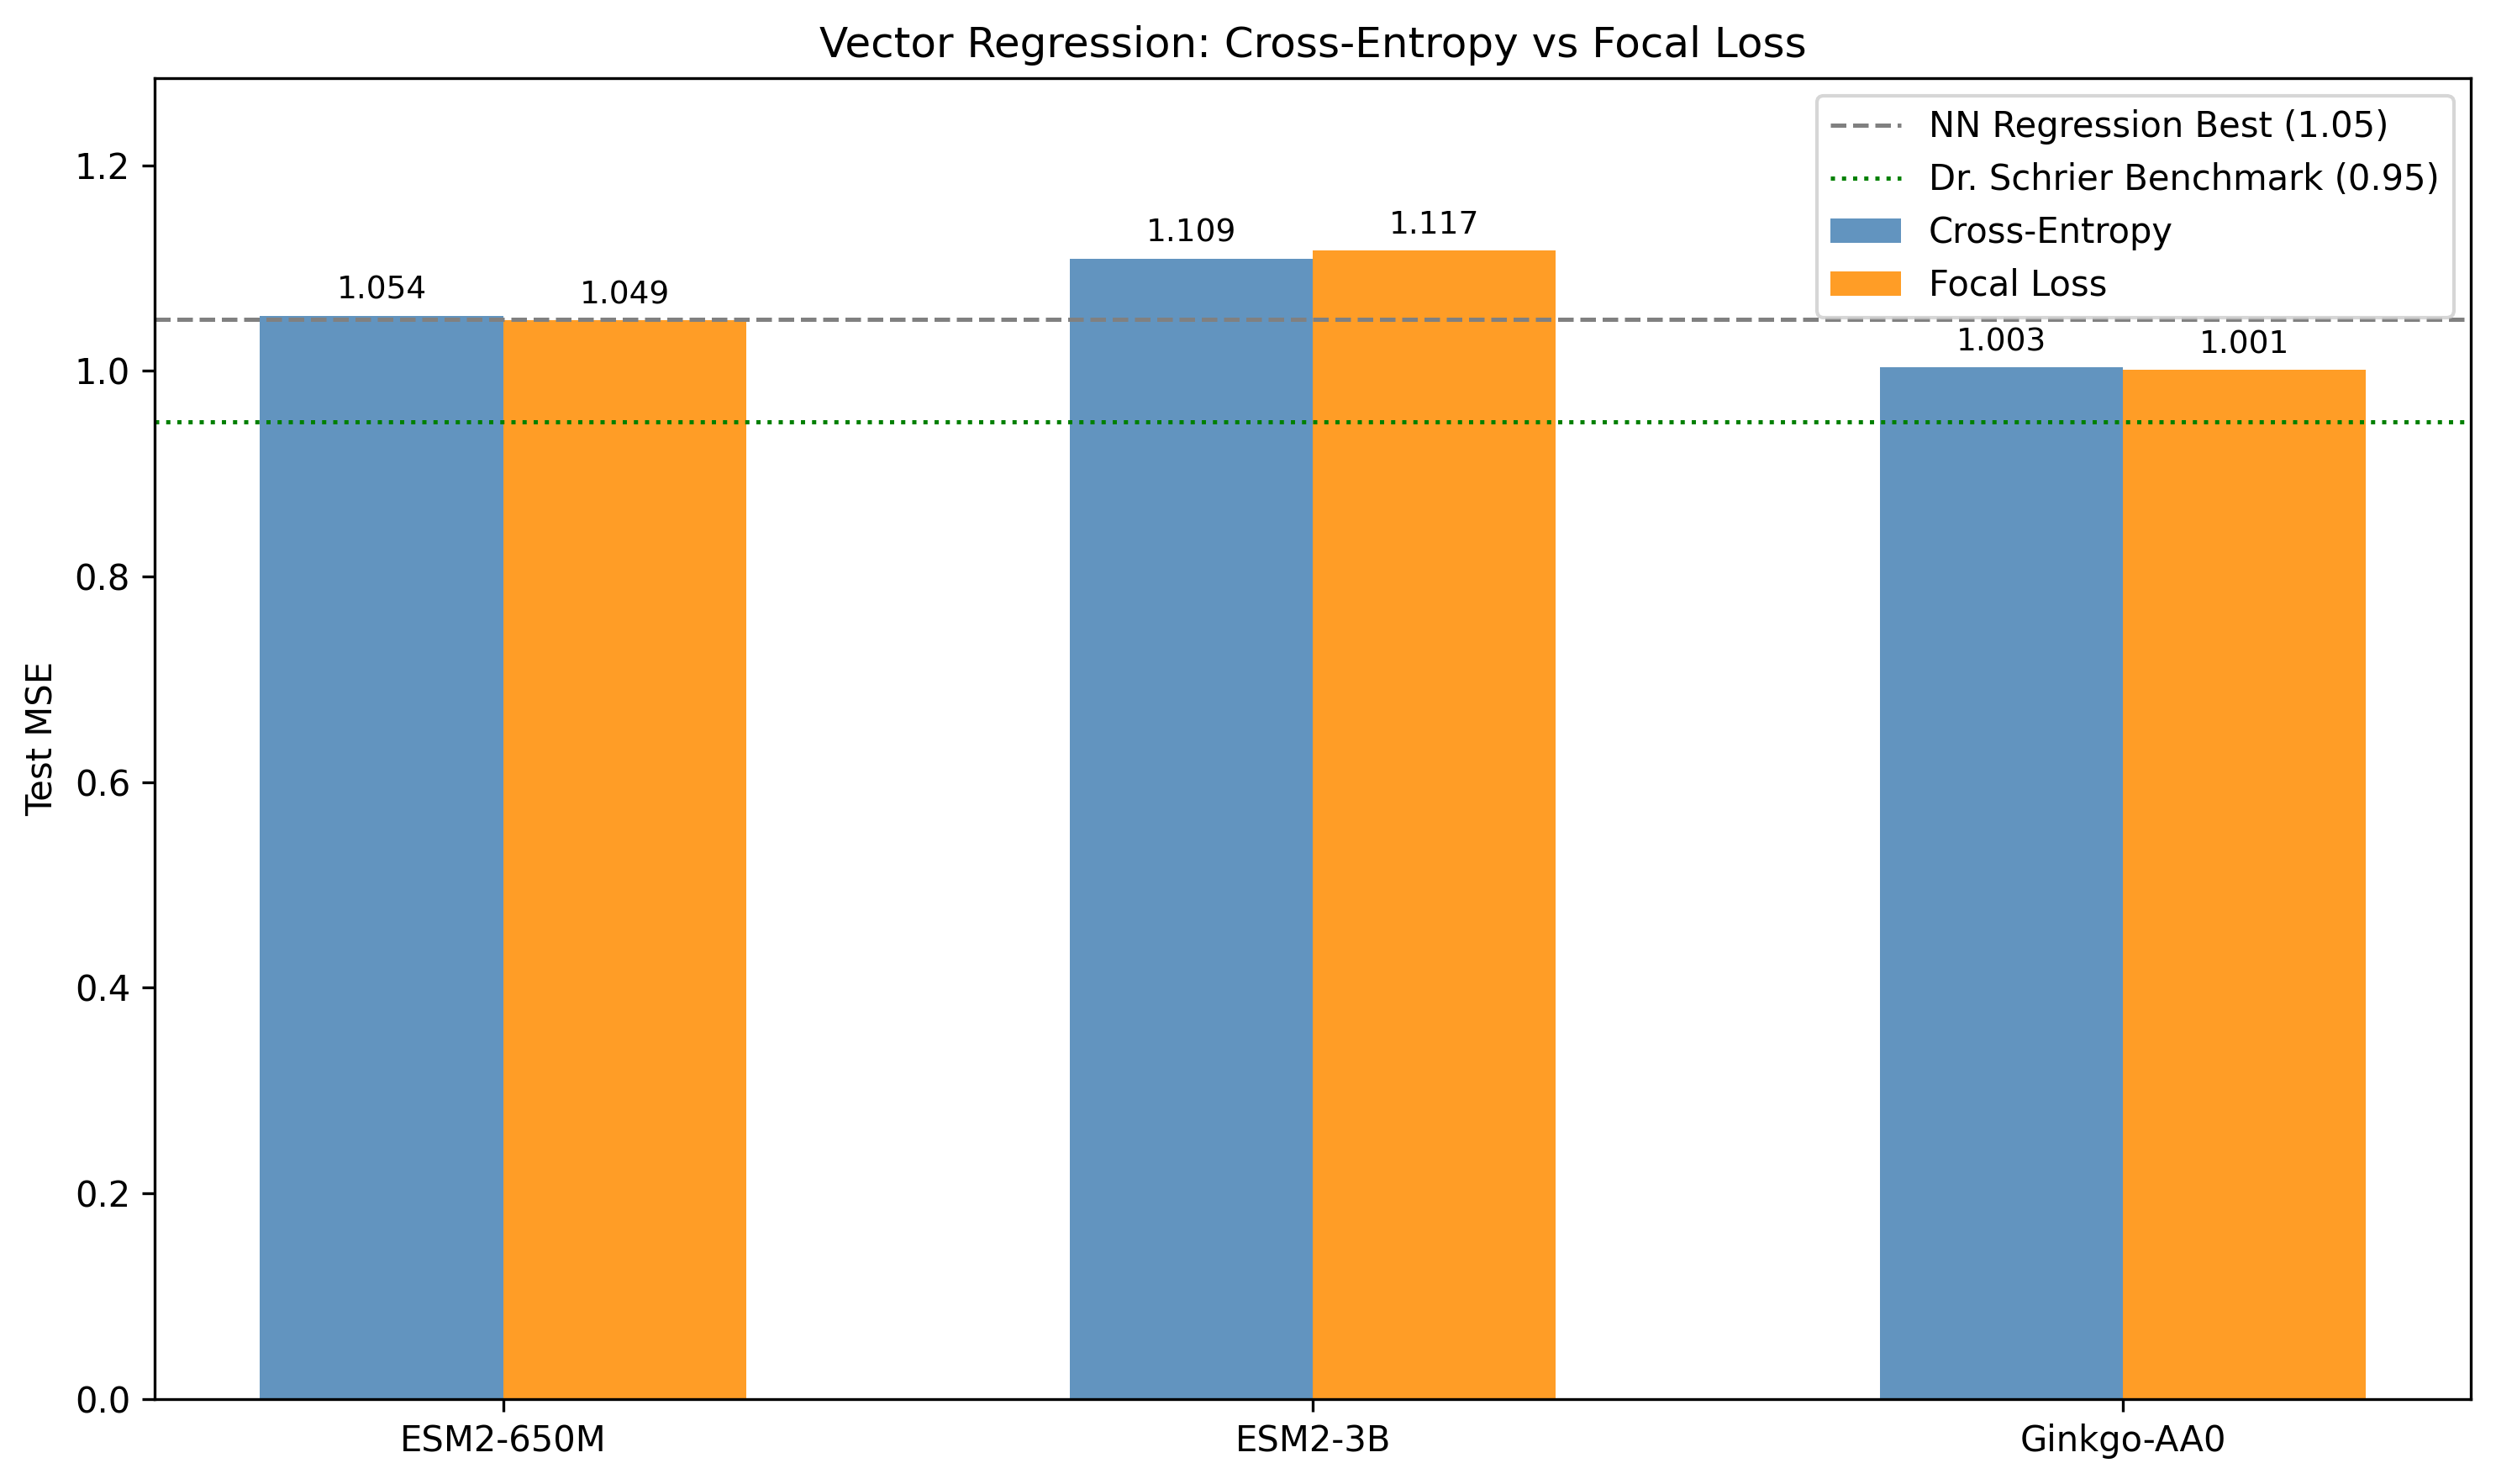
\includegraphics[width=0.95\textwidth]{../figures/vector_regression_comparison.png}
    \caption{Vector regression results comparing three PLM embedding types and two loss functions. Ensemble MSE values are annotated above each bar.}
    \label{fig:vector}
\end{figure}

\paragraph{Architecture and regularization optimization.}
\label{sec:fulldata_results}

While the base vector model improves over scalar regression, it still does not reach the 0.953 benchmark.
Table~\ref{tab:fulldata} presents results from the full-data optimization described in Section~\ref{sec:vector}.

\begin{table}[H]
\centering
\caption{Full-data vector regression optimization ($N_{\text{train}} = 3068$, $N_{\text{test}} = 1326$, Ginkgo-AA0 + focal loss). All results are 5-seed ensembles except where noted.}
\label{tab:fulldata}
\begin{tabular}{llcccc}
\toprule
Phase & Configuration & Dropout & Test MSE & Test $R^2$ & Spearman $\rho$ \\
\midrule
\multirow{3}{*}{Dropout}
 & (256, 256, 128), drop = 0.25 & 0.25 & 0.971 & --- & --- \\
 & (256, 256, 128), drop = 0.30 & 0.30 & 0.940 & --- & --- \\
 & (256, 256, 128), drop = 0.35 & 0.35 & \textbf{0.932} & \textbf{0.804} & \textbf{0.873} \\
\midrule
\multirow{2}{*}{4-layer}
 & (256, 256, 128, 64) & 0.20 & 0.940 & --- & --- \\
 & (384, 384, 256, 128) & 0.20 & 0.948 & --- & --- \\
\midrule
Mixed & 3-arch $\times$ 5-seed (15 models) & --- & 0.967 & --- & --- \\
\bottomrule
\end{tabular}
\end{table}

Dropout tuning produces the largest gains: increasing dropout from 0.20 to 0.35 on the (256, 256, 128) architecture reduces ensemble MSE from 0.993 to 0.932, indicating that the base configuration was under-regularized.
The best result, MSE 0.932 ($R^2 = 0.804$, Spearman $\rho = 0.873$), surpasses the prior benchmark of 0.953 by 2.2\%.
Bootstrap 95\% confidence intervals for this model are [0.823, 1.054] for MSE and [0.857, 0.887] for Spearman $\rho$ (Appendix~\ref{app:bootstrap}).
Four-layer architectures and mixed-architecture ensembles also beat the 0.953 benchmark but do not surpass the dropout-tuned 3-layer model.
Increasing to 20-seed ensembles does not improve over 5-seed, suggesting diminishing returns from additional ensemble members.

Figure~\ref{fig:ensemble_opt} shows the full optimization landscape.

\begin{figure}[H]
    \centering
    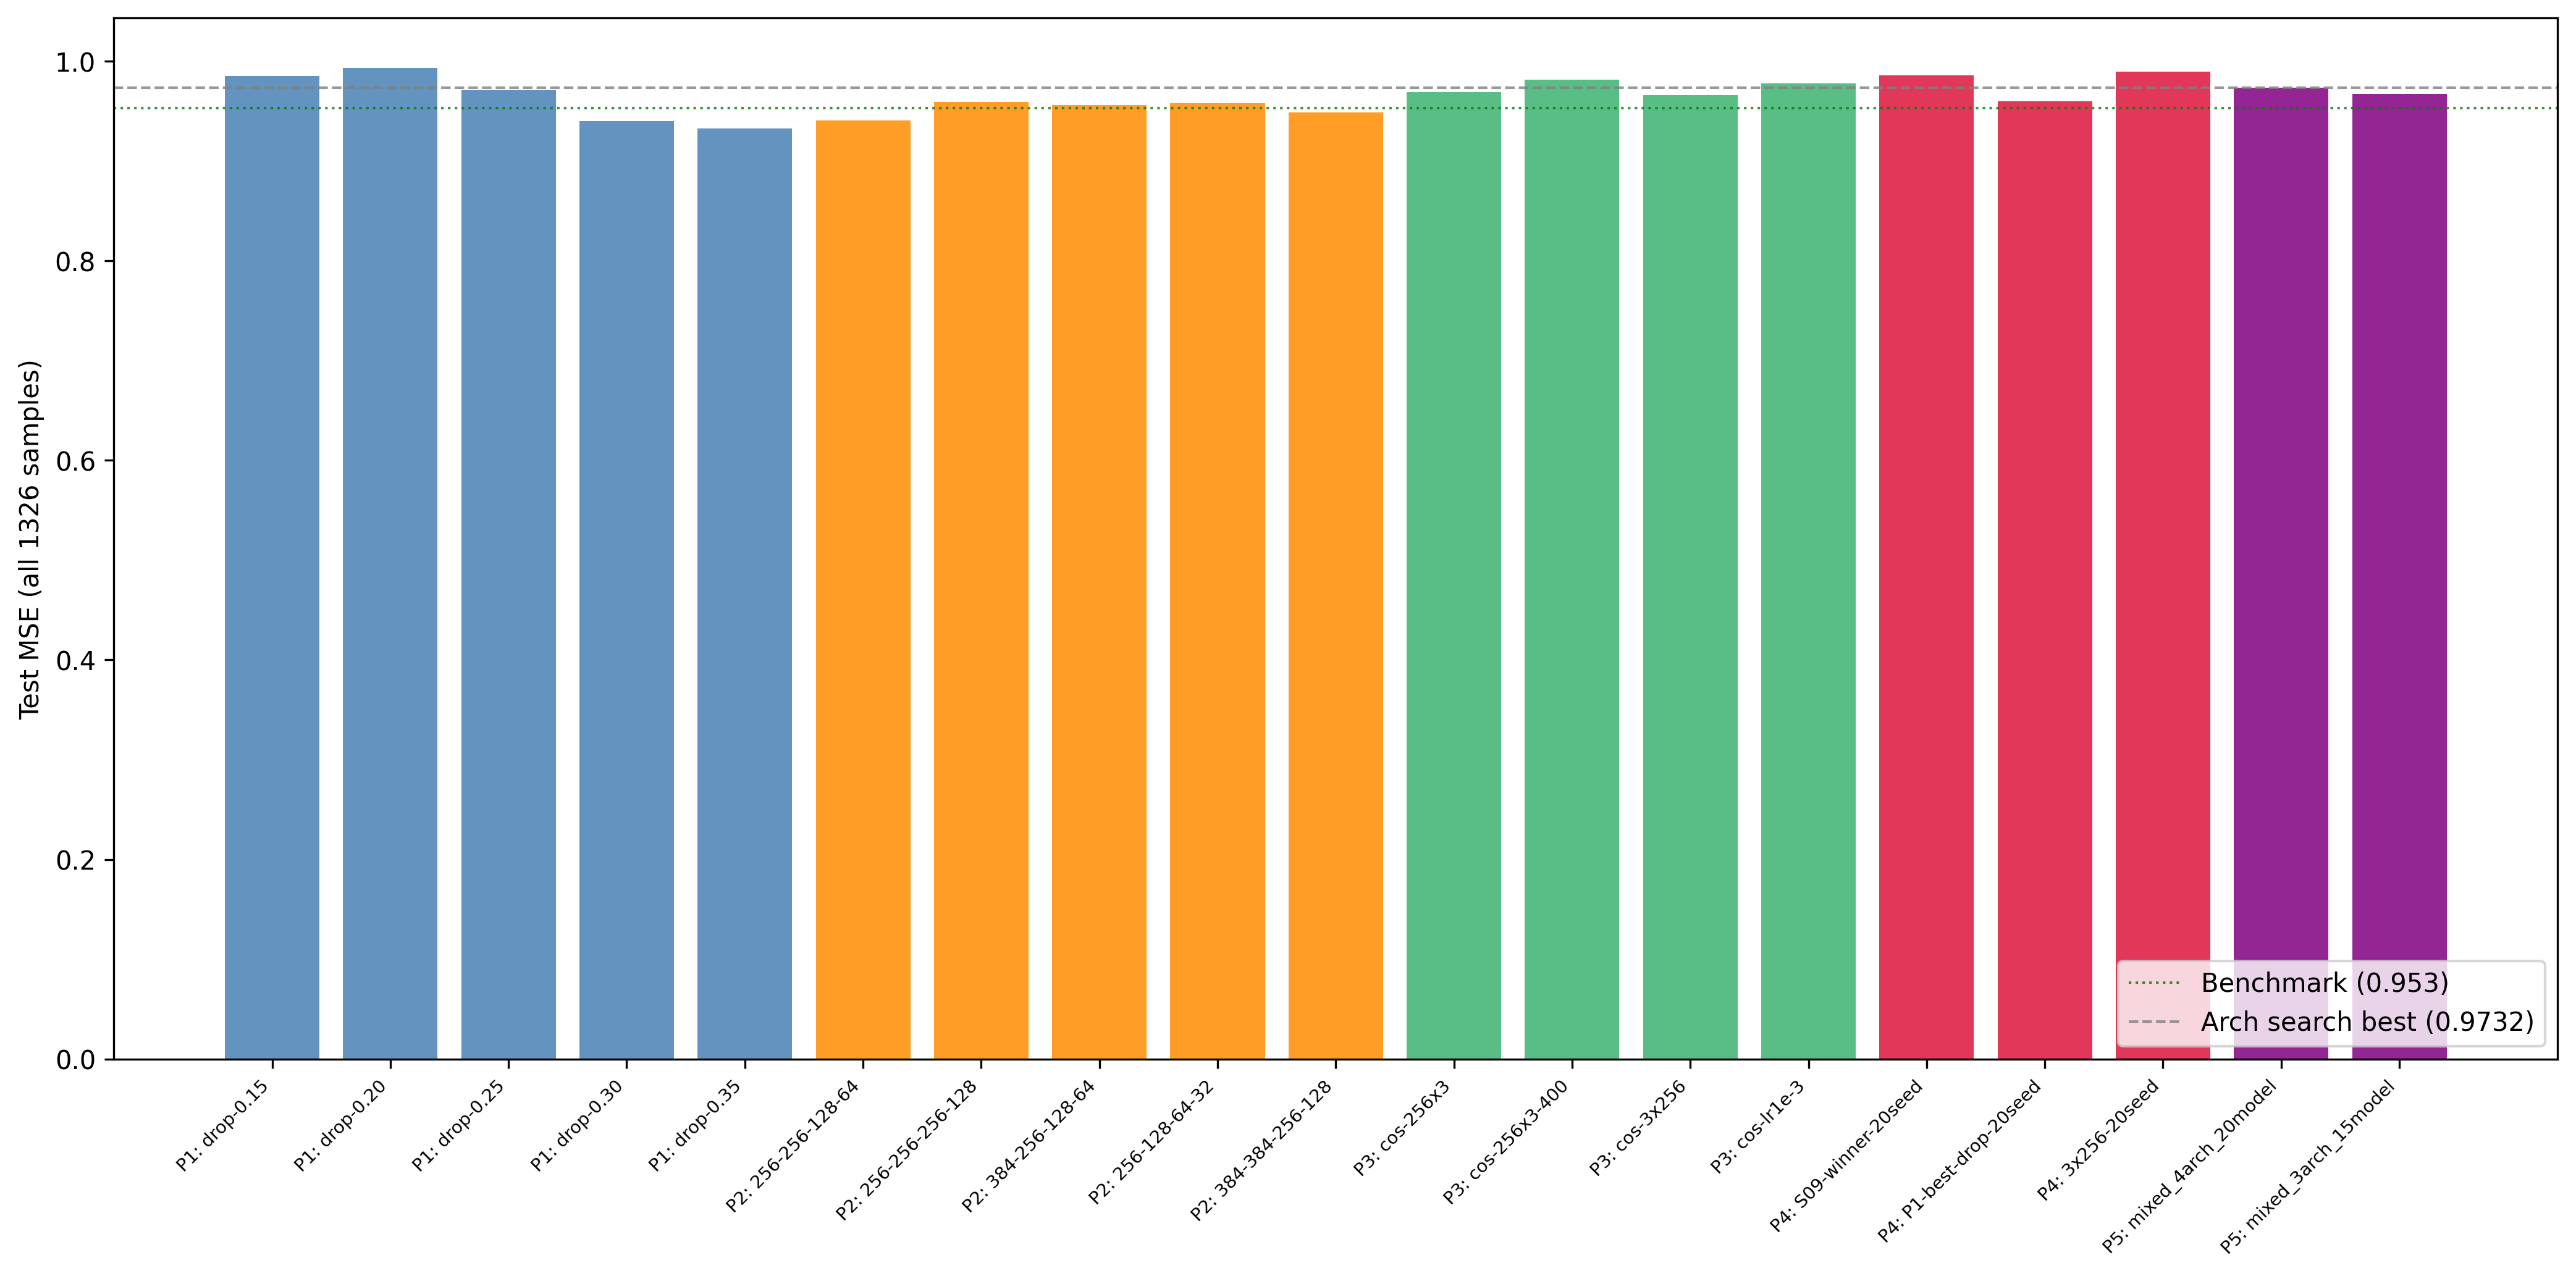
\includegraphics[width=0.95\textwidth]{../figures/vector_ensemble_optimization.png}
    \caption{Full-data vector regression optimization results. Configurations are grouped by optimization phase; the dotted green line indicates the prior benchmark of 0.953; the dashed grey line shows the Script~09 best (0.973).}
    \label{fig:ensemble_opt}
\end{figure}

\subsection{Cross-Dataset Generalization}
\label{sec:cross_results}

Table~\ref{tab:cross} summarizes cross-dataset performance for the best ESM2-650M RF and 5-seed NN ensemble.

\begin{table}[H]
\centering
\caption{Cross-dataset generalization. Models trained on Grasso data are evaluated on four external datasets. All Spearman correlations are significantly negative.}
\label{tab:cross}
\begin{tabular}{lrcrcr}
\toprule
Dataset & $N$ & \multicolumn{2}{c}{RF Spearman ($p$)} & \multicolumn{2}{c}{NN Spearman ($p$)} \\
\midrule
Wu & 81 & $-$0.314 & (0.004) & $-$0.241 & (0.030) \\
Xue & 322 & $-$0.278 & ($<$0.001) & $-$0.154 & (0.006) \\
Zhang-P43 & 114 & $-$0.218 & (0.020) & $-$0.196 & (0.037) \\
Zhang-PglVM & 114 & $-$0.250 & (0.007) & $-$0.213 & (0.023) \\
\bottomrule
\end{tabular}
\end{table}

All four external datasets yield statistically significant negative Spearman correlations for both RF and NN models.
For the Zhang datasets, where the same 114 signal peptides are measured under two promoters (P43 and PglVM), the model predictions achieve perfect rank consistency between the two promoter conditions (consistency = 1.000), while the actual WA measurements correlate at $r = 0.977$ across promoters.
Figure~\ref{fig:cross} visualizes the cross-dataset evaluation.

\begin{figure}[H]
    \centering
    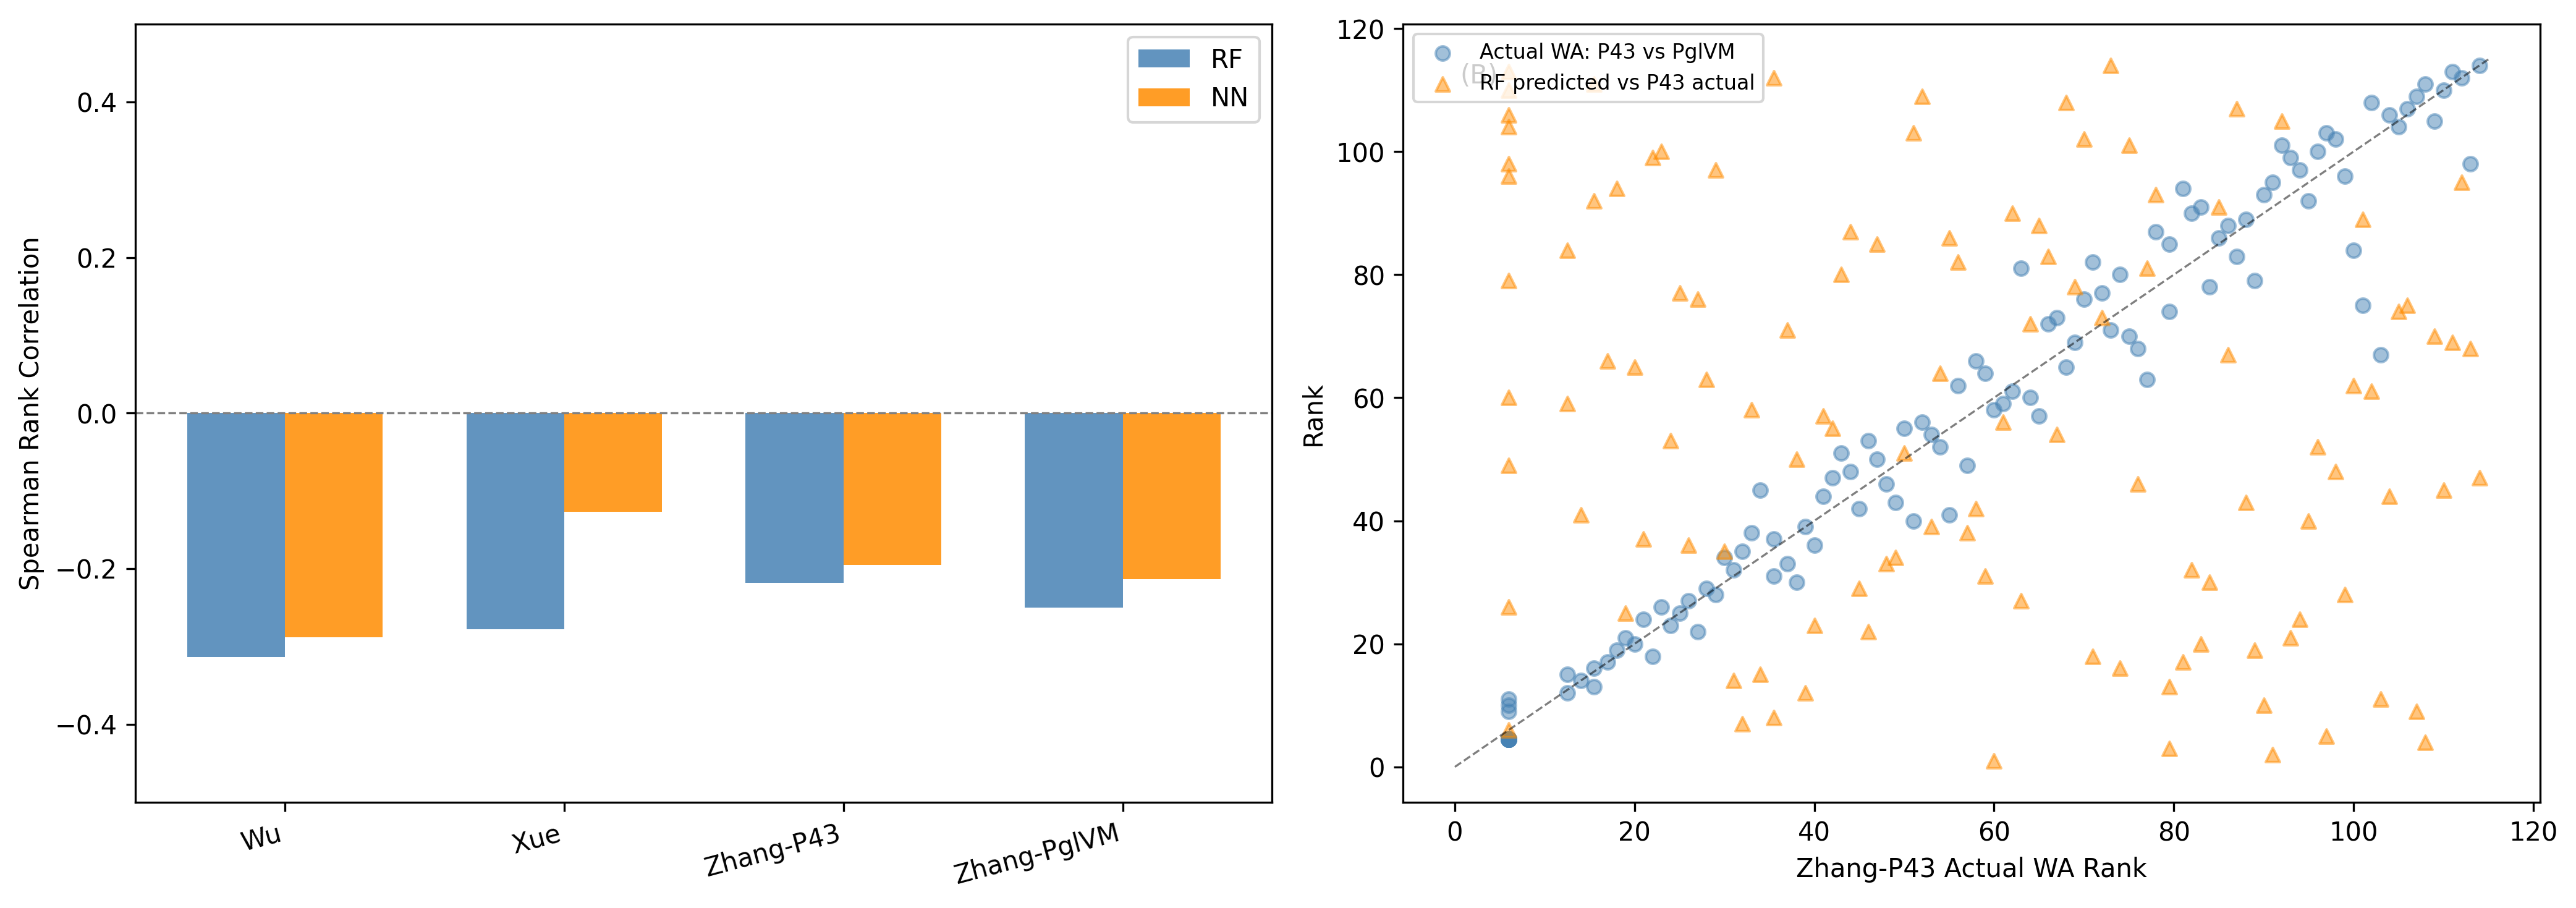
\includegraphics[width=0.95\textwidth]{../figures/cross_dataset_generalization.png}
    \caption{Cross-dataset generalization results. Spearman correlations between predicted and observed signal peptide efficiency across four external datasets. Error bars indicate 95\% confidence intervals.}
    \label{fig:cross}
\end{figure}

\paragraph{Fine-tuning results.}
Given the uniformly negative zero-shot correlations, we next test whether fine-tuning
the pretrained vector ensemble can recover positive transfer.
Table~\ref{tab:finetune} compares zero-shot and fine-tuned performance on each external dataset.

\begin{table}[H]
\centering
\caption{Cross-dataset fine-tuning results. The pretrained vector regression ensemble is
fine-tuned on each external dataset using 5-fold CV $\times$ 5 seeds. Zero-shot uses the
vector model directly; fine-tuned replaces and retrains the output head.}
\label{tab:finetune}
\begin{tabular}{lrcc}
\toprule
Dataset & $N$ & Zero-Shot $\rho$ & Fine-Tuned $\rho$ \\
\midrule
Wu & 81 & $-$0.181 & $+$0.193 $\pm$ 0.071 \\
Xue & 322 & $-$0.052 & $+$0.121 $\pm$ 0.083 \\
Zhang-P43 & 114 & $-$0.254 & $+$0.034 $\pm$ 0.154 \\
Zhang-PglVM & 114 & $-$0.282 & $-$0.040 $\pm$ 0.051 \\
\bottomrule
\end{tabular}
\end{table}

Fine-tuning reverses the negative zero-shot correlations for Wu and Xue, shifting
Spearman $\rho$ from $-$0.181 to $+$0.193 and from $-$0.052 to $+$0.121, respectively.
For the Zhang datasets, fine-tuning moves correlations toward zero ($-$0.254 $\to$ $+$0.034
for P43; $-$0.282 $\to$ $-$0.040 for PglVM) but does not achieve positive transfer,
likely due to the small training set (91--92 samples per fold) and the fundamental
biological differences between the Grasso and Zhang experimental systems.
The high variance across folds (e.g., Zhang-P43 $\pm$ 0.154) reflects the instability
of fine-tuning on small datasets.
Figure~\ref{fig:finetune} visualizes the zero-shot to fine-tuned improvement.

\begin{figure}[H]
    \centering
    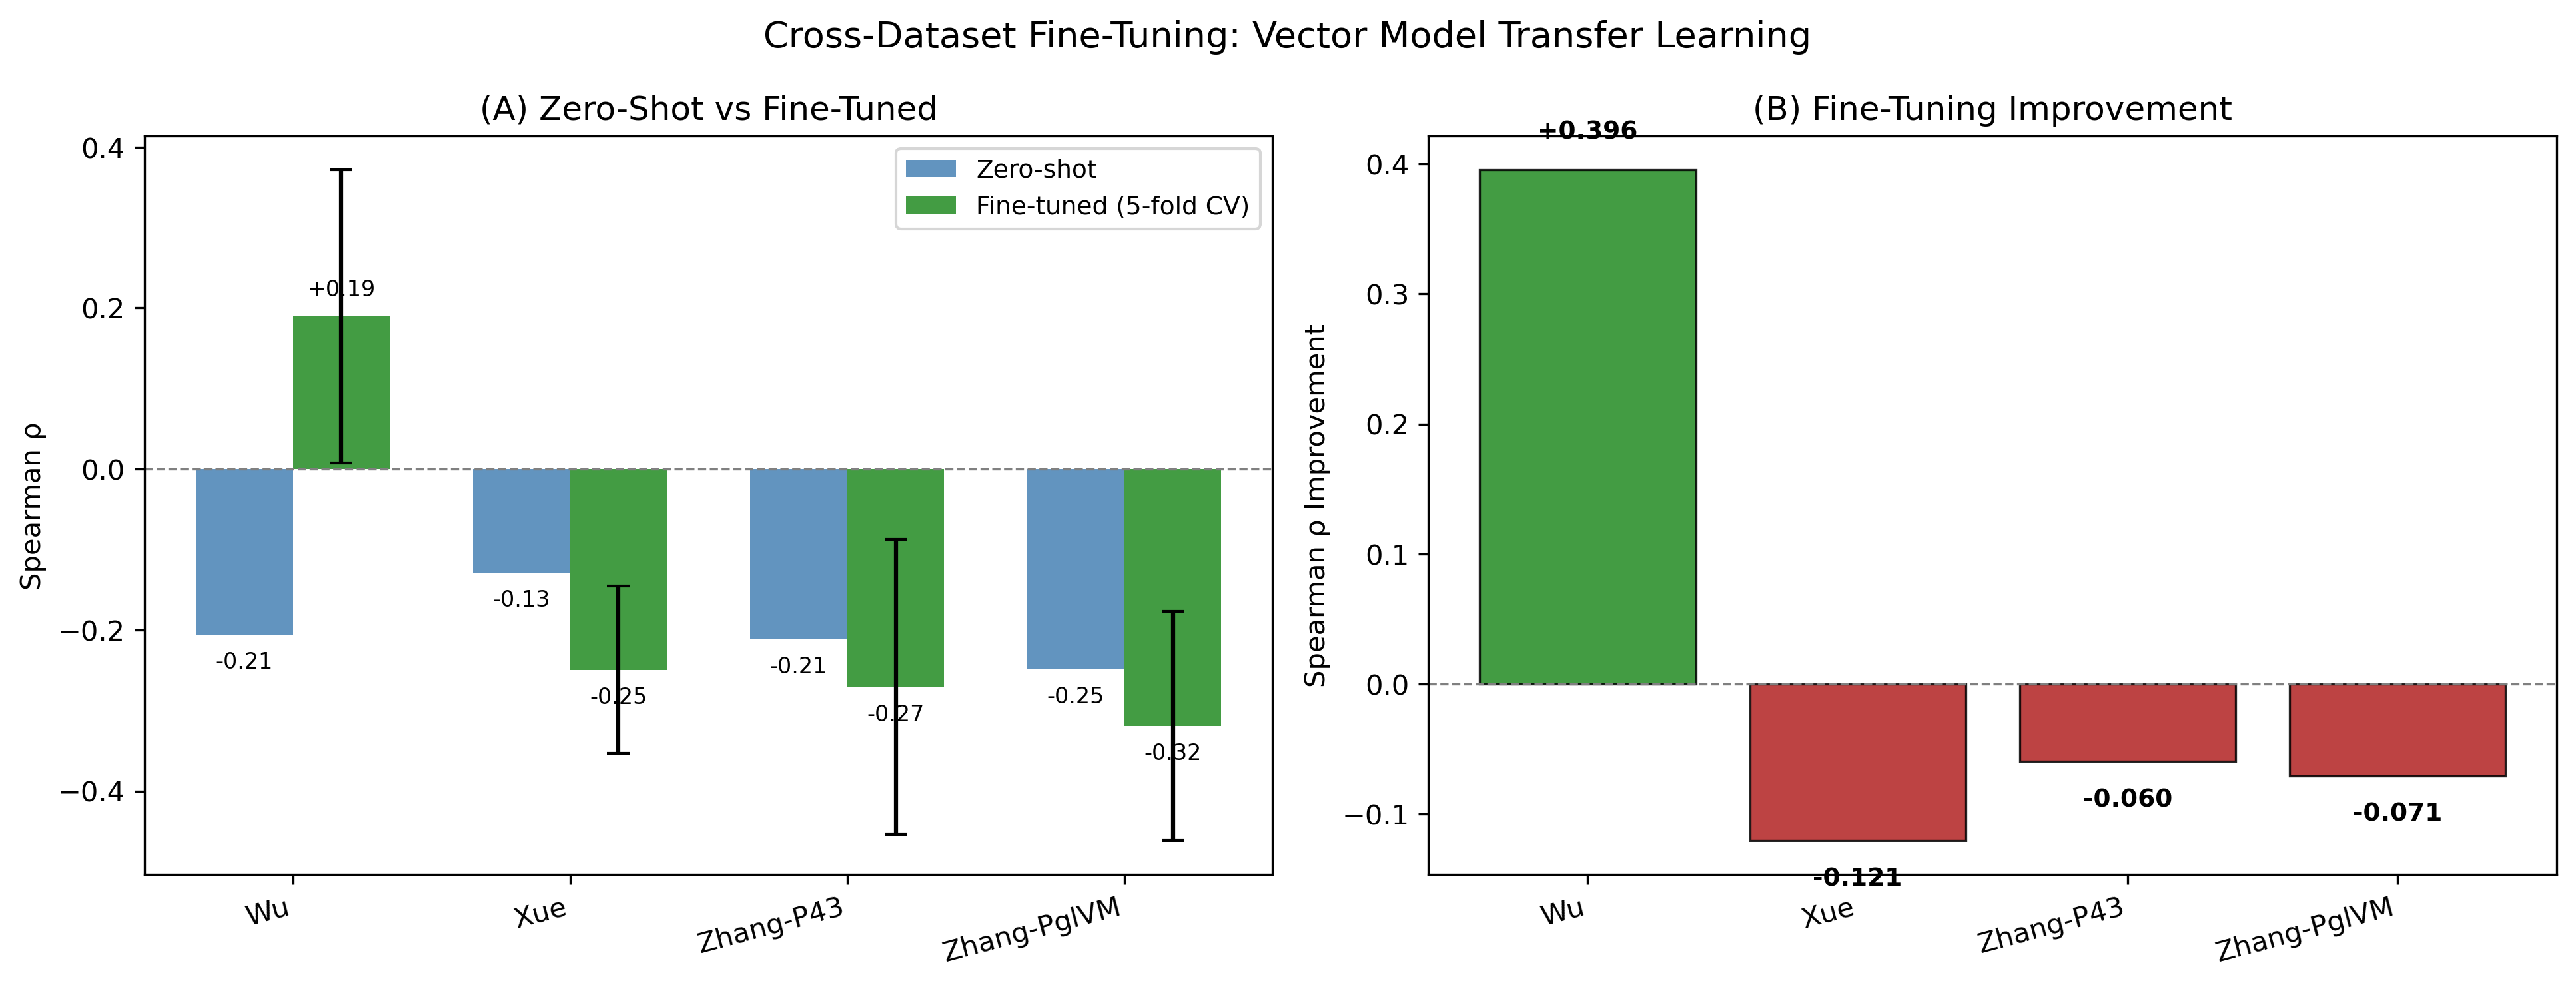
\includegraphics[width=0.95\textwidth]{../figures/cross_dataset_finetuning.png}
    \caption{Cross-dataset fine-tuning results. Zero-shot (red) vs.\ fine-tuned (blue) Spearman
    correlations for the vector regression ensemble on four external datasets. Error bars on
    fine-tuned values show standard deviation across 5-fold CV $\times$ 5 seeds.}
    \label{fig:finetune}
\end{figure}

\subsection{Design Task Evaluation}
\label{sec:design_results}

Beyond generalization to external datasets, we also evaluate whether the models can guide the design of new signal peptide variants within the Grasso system.
Table~\ref{tab:design} summarizes model performance on ranking 4832 designed signal peptide variants across 131 genes (of 134 total, after requiring $\geq$5 variants per gene).

\begin{table}[H]
\centering
\caption{Design task evaluation across two feature representations. Models predict relative performance of designed signal peptide variants compared to wild type.}
\label{tab:design}
\begin{tabular}{llcccc}
\toprule
Features & Model & Spearman $\rho$ & Pearson $r$ & MSE & ClassAcc (\%) \\
\midrule
ESM2-650M (1280d) & NN & \textbf{0.394} & \textbf{0.406} & 4.03 & 71.7 \\
PhysChem (156d) & NN & 0.386 & 0.400 & \textbf{3.99} & 72.0 \\
PhysChem (156d) & RF & 0.369 & 0.378 & 4.07 & \textbf{74.2} \\
ESM2-650M (1280d) & RF & 0.363 & 0.367 & 4.15 & 72.9 \\
\bottomrule
\end{tabular}
\end{table}

All four models achieve Spearman correlations above 0.36 and classification accuracy above 71\%, with all correlations significant at $p < 10^{-150}$.
The ESM2-650M NN achieves the highest rank correlation ($\rho = 0.394$), slightly outperforming the PhysChem NN (0.386), PhysChem RF (0.369), and ESM2-650M RF (0.363).
RF models achieve marginally better classification accuracy (74.2\% PhysChem, 72.9\% ESM2-650M) than NNs (71.7--72.0\%).
The improvement from ESM2-650M over PhysChem features is modest for the design task, consistent with the smaller RF--NN gap observed for scalar regression (Section~\ref{sec:results}).
Figure~\ref{fig:design} shows the design task results.

\begin{figure}[H]
    \centering
    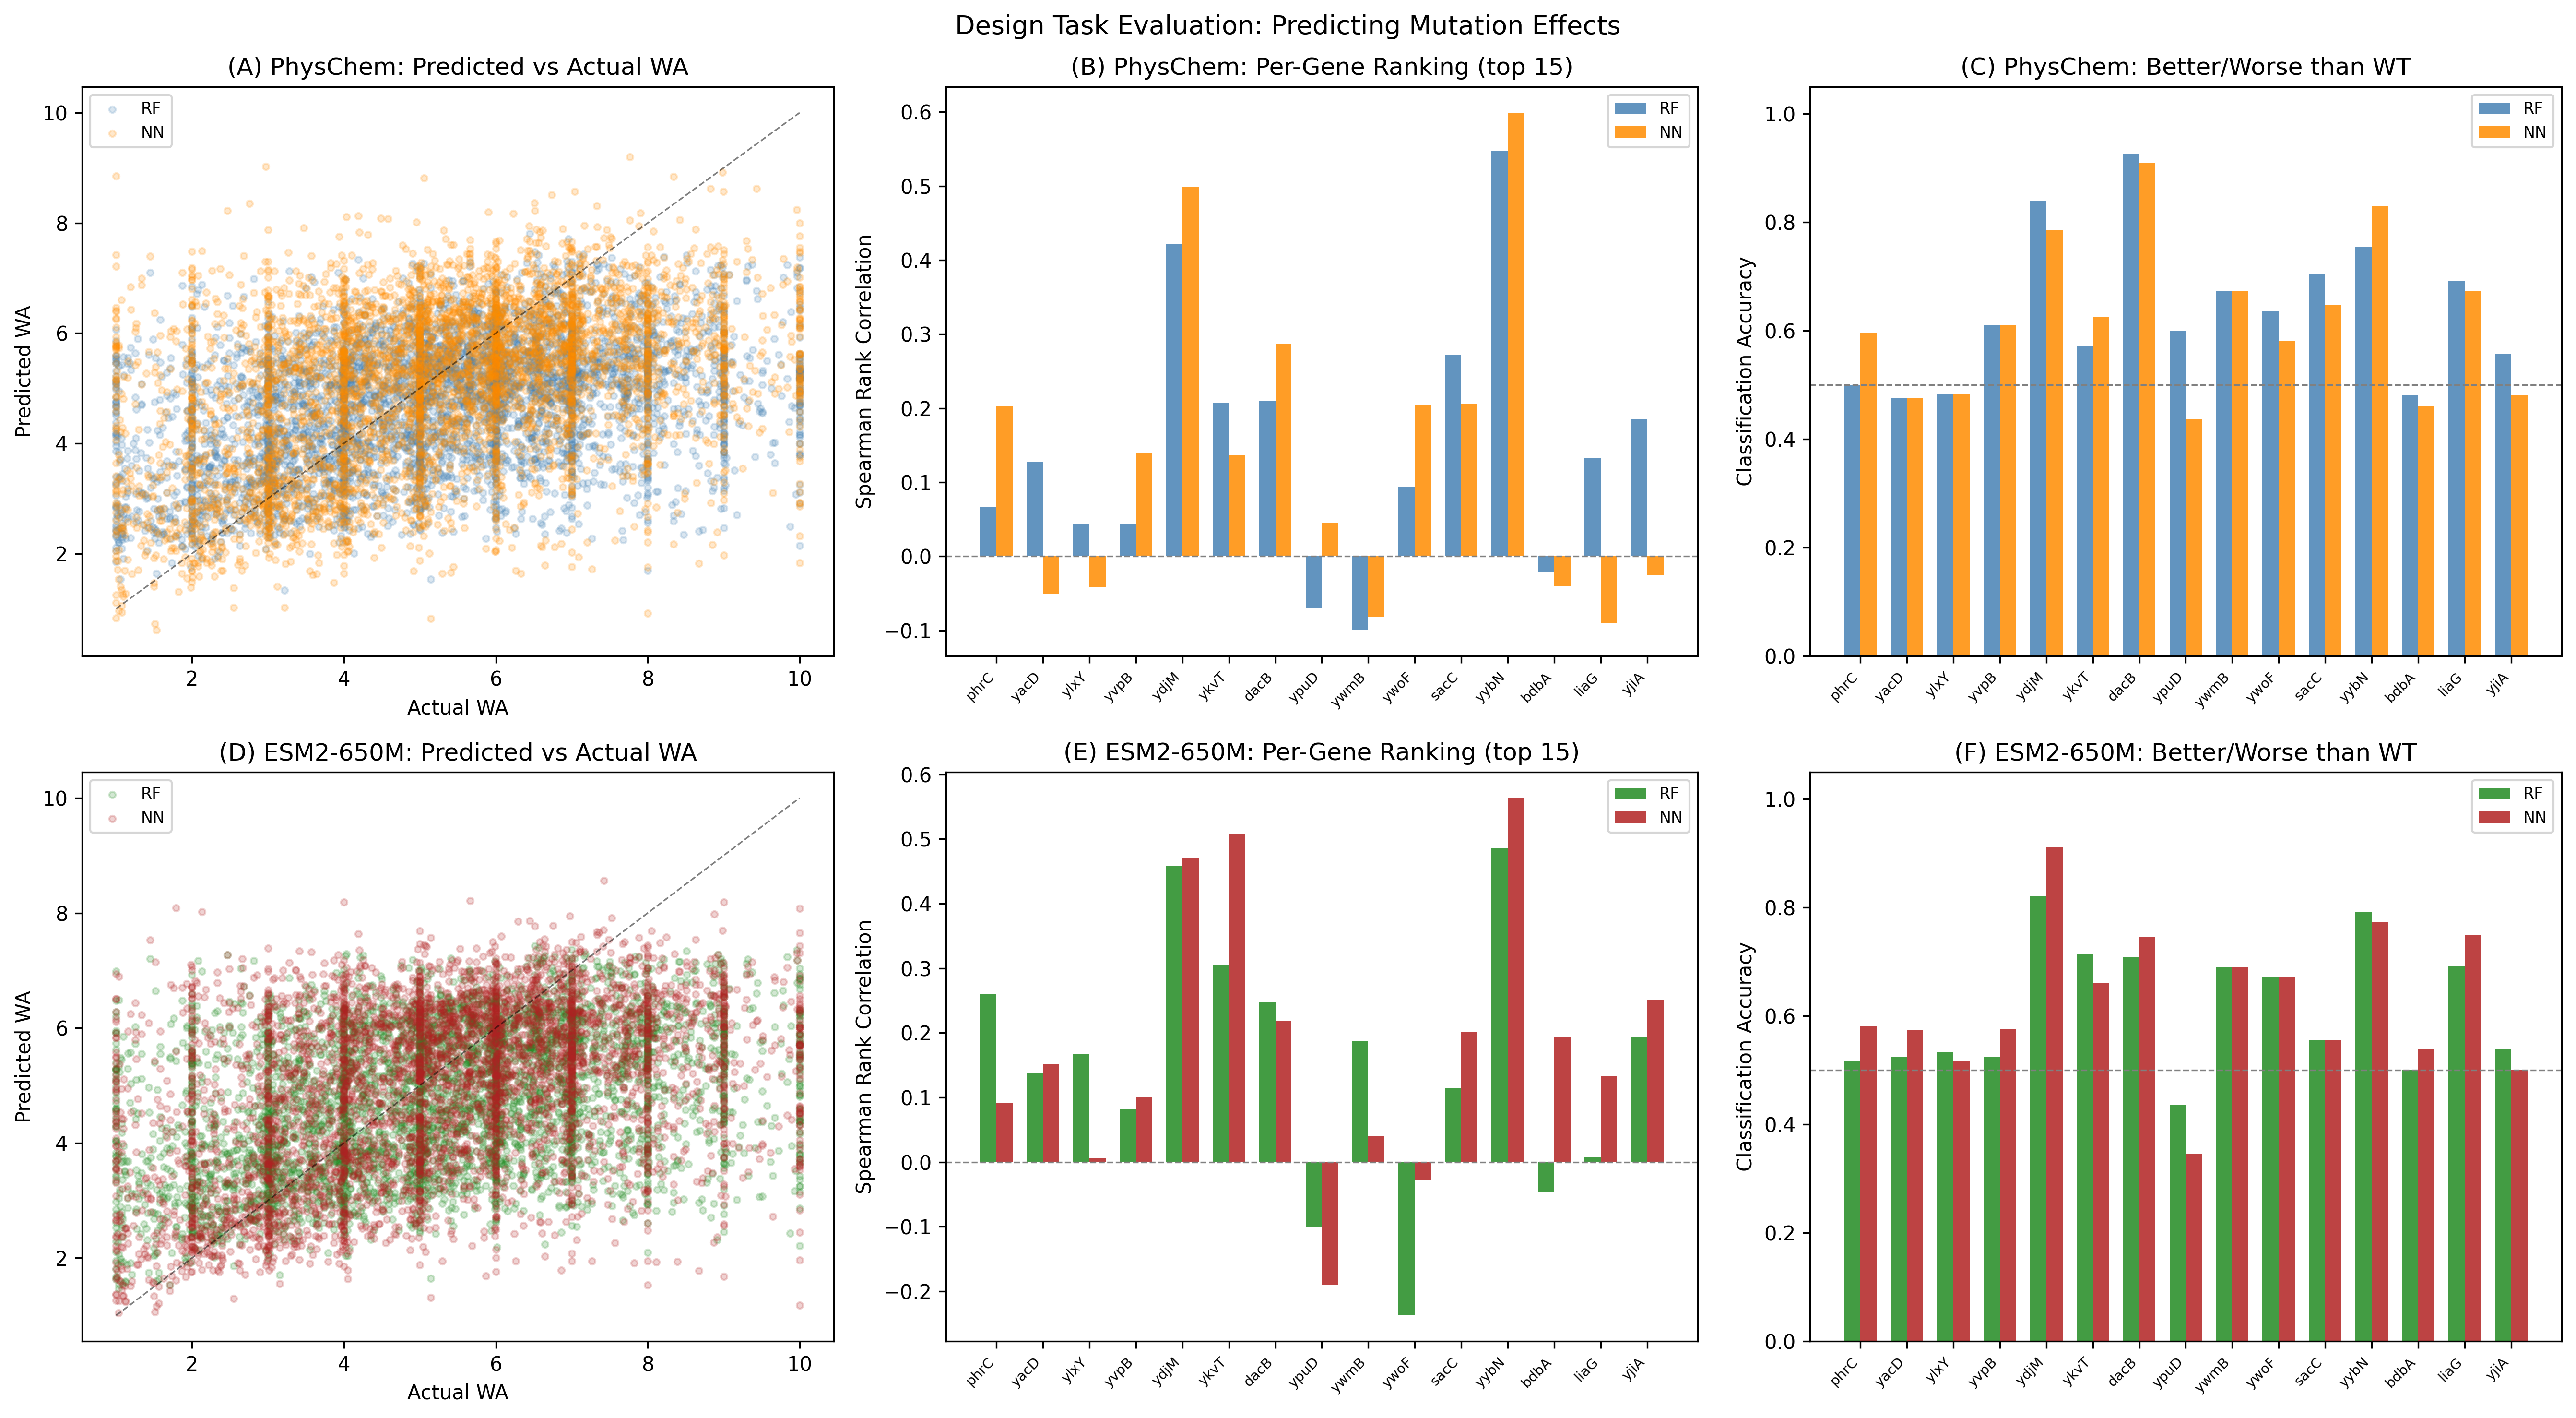
\includegraphics[width=0.95\textwidth]{../figures/design_task_evaluation.png}
    \caption{Design task evaluation. Model predictions for 4832 designed signal peptide variants across 131 genes (requiring $\geq$5 variants per gene), comparing physicochemical features (top row) and ESM2-650M embeddings (bottom row) with both RF and NN models.}
    \label{fig:design}
\end{figure}

% ══════════════════════════════════════════════════════════════════════════
\section{Discussion}
\label{sec:discussion}

\paragraph{Model--Representation Interaction.}
The central finding of the scalar regression analysis is a pronounced interaction between model architecture and feature representation.
Random forests show minimal sensitivity to input type; all four feature sets produce similar MSE values (1.16--1.25).
Neural networks, in contrast, exhibit a 27\% performance gap between the best (Ginkgo-AA0, MSE 1.050) and worst (PhysChem, MSE 1.328) feature types.

This pattern suggests that RF's built-in feature selection (via random subspace sampling) provides robustness to uninformative dimensions but limits the model's ability to exploit complex feature interactions.
Neural networks can learn nonlinear combinations of PLM embedding dimensions that capture secretion-relevant information, but require sufficient input richness to outperform simpler methods.
The poor performance of NN on physicochemical features (MSE 1.328) deserves a closer look.
With only 156 input dimensions and $\sim$3000 training samples, the neural network may lack sufficient signal to learn useful representations beyond what the RF already captures through axis-aligned splits.
The higher capacity of the NN becomes a liability rather than an asset in this low-dimensional regime.

\paragraph{PLM Model Size.}
A related question is whether larger PLMs automatically produce better predictions.
Surprisingly, the largest PLM (ESM2-3B, 2560 dimensions) does not yield the best results.
For RF, ESM2-3B performs worst among all models.
For NN, ESM2-3B (MSE 1.067) outperforms ESM2-650M (1.090) but is still outperformed by Ginkgo-AA0 (1.050).
With only $\sim$3000 training samples, the additional dimensions of the 3B model may introduce noise without proportional signal.
The Ginkgo-AA0 model, despite having fewer parameters than ESM2-3B, may encode more task-relevant biological information for signal peptide function.

\paragraph{Vector Regression.}
Beyond the choice of input features, the regression formulation itself also matters.
Predicting bin probability distributions instead of scalar WA values yields a 4.7\% MSE improvement over the best scalar NN (1.050 $\to$ 1.001).
This gain likely arises from the richer supervision signal: each training example provides 10 target values instead of one, and the softmax output naturally enforces a valid probability distribution.
Focal loss provides a marginal improvement over cross-entropy, suggesting that most of the gain comes from the architectural change rather than the loss function.
However, the vector and scalar NNs also differ in activation function (LeakyReLU vs.\ ReLU) and the absence of batch normalization, so the improvement cannot be attributed solely to the distributional output without further ablation.
With an 80/20 validation split, the best vector model achieves MSE 1.001, above the 0.953 obtained using a near-identical architecture (same embedding, hidden sizes, dropout, and focal loss; Schrier uses parametric ReLU vs.\ our LeakyReLU) implemented in Wolfram Language (J.\ Schrier, personal communication).
Removing the validation split and optimizing dropout (0.35 vs.\ 0.20) with a deeper three-layer architecture (256, 256, 128) yields a 5-seed ensemble MSE of 0.932 (Section~\ref{sec:fulldata_results}), surpassing that benchmark by 2.2\%.
The key improvements are (i) an additional hidden layer providing greater model capacity, (ii) higher dropout regularization compensating for the absence of early stopping, and (iii) multi-seed ensembling to reduce prediction variance.

\paragraph{Cross-Dataset Generalization.}
While these improvements are substantial within the Grasso dataset, the cross-dataset results paint a different picture.
The consistently negative Spearman correlations across all four external datasets are worth examining, though not entirely unexpected.
Signal peptide efficiency depends on the cargo protein, promoter, host organism, and growth conditions, all of which differ fundamentally between datasets.
The correlations are not merely absent ($\rho \approx 0$) but actively negative, suggesting that the sequence features associated with high secretion in the Grasso system are associated with low performance in other contexts, possibly because the model has learned host- or cargo-specific signal patterns that are maladaptive elsewhere.
A signal peptide optimized for $\beta$-glucuronidase secretion in \textit{B.\ subtilis} may be poorly suited for xylanase production in the same organism, let alone for enzyme secretion in \textit{E.\ coli} or \textit{S.\ cerevisiae}.
The Zhang cross-promoter analysis provides complementary evidence: the same 114 signal peptides correlate at $r = 0.977$ across two promoters, confirming that signal peptide rankings are partially conserved within a system but not across systems.
In practice, this means models for signal peptide optimization need to be trained on task-specific data rather than transferred across experimental contexts.
Fine-tuning the pretrained vector ensemble on target-domain data partially addresses this
limitation: freezing the learned feature layers and retraining only the output head reverses
the negative correlations for Wu ($-$0.181 $\to$ $+$0.193) and Xue ($-$0.052 $\to$ $+$0.121),
demonstrating that the pretrained representations capture transferable signal peptide features
even when zero-shot predictions are anti-correlated.
However, the small Zhang datasets (114 samples, $\sim$91 per training fold) do not support
effective fine-tuning, underscoring that transfer learning for signal peptide efficiency remains
data-limited.

\paragraph{Design Task.}
Despite the limited cross-dataset transferability, the models still prove useful within the Grasso experimental system.
The design task demonstrates that models trained on characterized variants can meaningfully rank novel designed signal peptides, with Spearman $\rho = 0.36$--0.39 and classification accuracy of 72--74\%, well above the 50\% random baseline.
Generating ESM2-650M embeddings for the design variants and evaluating all four model--feature combinations reveals that the ESM2-650M NN achieves the highest rank correlation ($\rho = 0.394$), though the improvement over PhysChem features is modest (0.394 vs.\ 0.386 for NN, 0.363 vs.\ 0.369 for RF).
This contrasts with the larger PLM advantage observed in the scalar regression task, suggesting that the design task's evaluation structure (per-gene ranking rather than absolute WA prediction) may limit the benefit of richer representations.
The moderate but significant correlations suggest that these models can serve as a practical filter for prioritizing candidates in experimental screening campaigns.

\paragraph{Limitations.}
Several caveats apply to these findings.
The RF and NN hyperparameter searches used different validation strategies (5-fold CV vs.\ single train/val split), which may introduce some asymmetry in the comparison.
The dataset is limited to \textit{B.\ subtilis} with a single reporter enzyme.
While full-data training with optimized regularization (MSE 0.932) surpasses the prior benchmark of 0.953, this result relies on a 5-seed ensemble and training without a validation split, which precludes early stopping.
To verify that the dropout selection is not an artifact of test-set model selection, we repeated the dropout sweep with an independent 80/20 train/validation split (Appendix~\ref{app:dropout_val}).
Validation MSE decreases from 1.384 at dropout 0.15 to 1.341 at dropout 0.30, confirming that higher dropout improves generalization; the validation-optimal (0.30) and test-optimal (0.35) dropouts are adjacent and statistically indistinguishable on held-out data.
The differences between top-performing models are modest; 95\% bootstrap confidence intervals for all models are reported in Appendix~\ref{app:bootstrap}.
The cross-dataset significance tests (Table~\ref{tab:cross}) involve eight comparisons; after Bonferroni correction ($\alpha = 0.00625$), three of the four NN correlations and two of the four RF correlations no longer reach significance. The Wu and Xue datasets retain significant RF correlations, and only Xue retains a significant NN correlation.
The vector regression architecture uses LeakyReLU activation and omits batch normalization,
while the scalar NN uses ReLU with batch normalization; a systematic ablation of these
architectural differences was not performed, so the vector regression improvement cannot
be attributed solely to the distributional output.
Ginkgo-AA0 embeddings, which yielded the best results across all tasks, were only
available for the Grasso dataset; cross-dataset and fine-tuning evaluations use ESM2-650M
embeddings, so the actual transferability of Ginkgo-AA0 representations remains untested.

% ══════════════════════════════════════════════════════════════════════════
\section{Conclusion}
\label{sec:conclusion}

We have systematically evaluated signal peptide efficiency prediction across four feature representations, two model architectures, and two regression formulations.
A vector regression neural network with Ginkgo-AA0 embeddings and focal loss achieves MSE 1.001 ($R^2 = 0.790$) with validation-based training.
Full-data optimization with increased dropout and a deeper architecture yields a 5-seed ensemble MSE of 0.932 ($R^2 = 0.804$, Spearman $\rho = 0.873$), improving 23.6\% over the physicochemical baseline of 1.22 and surpassing the prior benchmark of 0.953 by 2.2\%.
Cross-dataset evaluation reveals that zero-shot predictions do not generalize across organisms or experimental systems, but fine-tuning the output head on target-domain data reverses the negative correlations for two of four datasets, suggesting the pretrained representations encode partially transferable signal peptide features.
Applied to designed variants using both physicochemical and ESM2-650M features, the models achieve classification accuracy of 72--74\% and Spearman $\rho$ up to 0.394, demonstrating practical utility for guiding experimental prioritization.

Random forests remain competitive and robust across feature types, making them suitable when interpretability or computational efficiency is prioritized.
These results demonstrate that realizing the potential of protein language models for biological prediction tasks requires appropriate model architectures; simply replacing hand-crafted features with PLM embeddings does not guarantee improvement.
Future work could explore ensemble methods combining RF and NN predictions, end-to-end fine-tuning of PLM weights on secretion efficiency data, or extending the analysis to additional host organisms and cargo proteins.

% ══════════════════════════════════════════════════════════════════════════
\section*{Data Availability}

The original dataset is available as supplementary material to \citet{grasso2023}.
PLM embeddings were generated using publicly available model weights.
All analysis code and results are available at \url{https://github.com/Mehak-W/signal-peptide-experiments}.

% ══════════════════════════════════════════════════════════════════════════
\bibliographystyle{unsrtnat}
\bibliography{references}

% ══════════════════════════════════════════════════════════════════════════
\appendix

% ── Appendix A: Hyperparameter Search Results ─────────────────────────────
\section{Hyperparameter Search Results}
\label{app:hyperparam}

Tables~\ref{tab:rf_trials} and \ref{tab:nn_trials} report the top-10 configurations per feature type from the randomized hyperparameter searches (100 RF configs with 5-fold CV; 40 NN configs with 80/20 validation split).
Full trial data are available in the GitHub repository.

\begin{table}[H]
\centering
\caption{Top-5 random forest configurations per feature type, ranked by 5-fold cross-validation MSE (100 configs searched per type).}
\label{tab:rf_trials}
\small
\begin{tabular}{clccccc}
\toprule
Feature & Rank & $n_{\text{est}}$ & Depth & Split & Leaf & CV MSE \\
\midrule
\multirow{5}{*}{PhysChem}
 & 1 & 75 & None & 5 & 2 & 2.019 \\
 & 2 & 50 & 25 & 2 & 1e-4 & 2.021 \\
 & 3 & 150 & 30 & 2 & 1e-4 & 2.028 \\
 & 4 & 100 & 30 & 10 & 1e-3 & 2.029 \\
 & 5 & 150 & 25 & 2 & 2 & 2.029 \\
\midrule
\multirow{5}{*}{ESM2-650M}
 & 1 & 300 & 25 & 1e-3 & 4 & 1.843 \\
 & 2 & 200 & 20 & 2 & 1e-3 & 1.845 \\
 & 3 & 300 & None & 10 & 4 & 1.845 \\
 & 4 & 75 & 25 & 5 & 1e-3 & 1.847 \\
 & 5 & 200 & 20 & 2 & 4 & 1.847 \\
\midrule
\multirow{5}{*}{ESM2-3B}
 & 1 & 150 & 25 & 2 & 2 & 1.925 \\
 & 2 & 300 & 25 & 1e-3 & 4 & 1.927 \\
 & 3 & 100 & 30 & 10 & 1e-3 & 1.928 \\
 & 4 & 200 & 25 & 2 & 1e-3 & 1.929 \\
 & 5 & 200 & 25 & 1e-3 & 1e-3 & 1.929 \\
\midrule
\multirow{5}{*}{Ginkgo-AA0}
 & 1 & 300 & None & 10 & 4 & 1.723 \\
 & 2 & 75 & None & 2 & 1e-4 & 1.723 \\
 & 3 & 150 & 30 & 2 & 1e-4 & 1.724 \\
 & 4 & 200 & 20 & 2 & 1e-3 & 1.724 \\
 & 5 & 100 & 25 & 2 & 2 & 1.725 \\
\bottomrule
\end{tabular}
\end{table}

\begin{table}[H]
\centering
\caption{Top-5 neural network configurations per feature type, ranked by validation MSE (40 configs searched per type, 80/20 train/val split).}
\label{tab:nn_trials}
\small
\begin{tabular}{clccccr}
\toprule
Feature & Rank & Layers & Drop & L2 & LR / Batch & Val MSE \\
\midrule
\multirow{5}{*}{PhysChem}
 & 1 & 256, 128 & 0.3 & 0.01 & 1e-3 / 64 & 1.390 \\
 & 2 & 128, 64 & 0.3 & 0.01 & 1e-3 / 32 & 1.425 \\
 & 3 & 128, 64 & 0.4 & 1e-4 & 1e-3 / 64 & 1.515 \\
 & 4 & 128, 64 & 0.5 & 0.01 & 5e-4 / 64 & 1.529 \\
 & 5 & 128, 64 & 0.4 & 1e-3 & 5e-4 / 64 & 1.551 \\
\midrule
\multirow{5}{*}{ESM2-650M}
 & 1 & 256, 128 & 0.4 & 0.01 & 1e-3 / 64 & 1.241 \\
 & 2 & 256 & 0.3 & 1e-3 & 5e-4 / 64 & 1.266 \\
 & 3 & 512, 256 & 0.5 & 0.01 & 5e-4 / 64 & 1.300 \\
 & 4 & 256, 128 & 0.5 & 1e-4 & 5e-4 / 64 & 1.331 \\
 & 5 & 256, 128 & 0.4 & 0.01 & 5e-4 / 32 & 1.353 \\
\midrule
\multirow{5}{*}{ESM2-3B}
 & 1 & 1024, 512 & 0.4 & 0.01 & 1e-3 / 64 & 1.302 \\
 & 2 & 512, 256 & 0.5 & 1e-3 & 1e-3 / 32 & 1.316 \\
 & 3 & 512, 256 & 0.4 & 1e-3 & 5e-4 / 32 & 1.333 \\
 & 4 & 512, 256 & 0.3 & 1e-3 & 1e-3 / 64 & 1.377 \\
 & 5 & 512, 256 & 0.2 & 0.01 & 5e-4 / 32 & 1.387 \\
\midrule
\multirow{5}{*}{Ginkgo-AA0}
 & 1 & 256, 128 & 0.3 & 1e-4 & 5e-4 / 32 & 1.146 \\
 & 2 & 512, 256 & 0.5 & 1e-3 & 5e-4 / 64 & 1.197 \\
 & 3 & 256 & 0.2 & 1e-3 & 1e-3 / 32 & 1.224 \\
 & 4 & 256, 128 & 0.5 & 1e-4 & 1e-3 / 64 & 1.236 \\
 & 5 & 256, 128 & 0.5 & 0.01 & 1e-3 / 32 & 1.248 \\
\bottomrule
\end{tabular}
\end{table}

% ── Appendix B: Vector Regression Per-Seed Results ────────────────────────
\section{Vector Regression Per-Seed Results}
\label{app:vector_seeds}

Table~\ref{tab:vector_seeds} reports the per-seed test MSE for all six embedding--loss combinations, along with the ensemble mean.

\begin{table}[H]
\centering
\caption{Per-seed test MSE for vector regression models. Each model uses the same architecture (2$\times$256 hidden units, LeakyReLU, 20\% dropout, softmax output) with 5 random seeds for train/validation splitting.}
\label{tab:vector_seeds}
\begin{tabular}{llcccccr}
\toprule
Embedding & Loss & Seed 42 & Seed 123 & Seed 456 & Seed 789 & Seed 1024 & Ensemble \\
\midrule
Ginkgo-AA0 & Focal & 1.026 & 1.120 & 1.023 & 1.128 & 1.046 & \textbf{1.001} \\
Ginkgo-AA0 & CE & 1.053 & 1.102 & 1.054 & 1.111 & 1.050 & 1.003 \\
ESM2-650M & Focal & 1.084 & 1.158 & 1.100 & 1.169 & 1.125 & 1.049 \\
ESM2-650M & CE & 1.084 & 1.151 & 1.093 & 1.194 & 1.132 & 1.054 \\
ESM2-3B & CE & 1.235 & 1.224 & 1.179 & 1.196 & 1.214 & 1.109 \\
ESM2-3B & Focal & 1.215 & 1.220 & 1.185 & 1.226 & 1.193 & 1.117 \\
\bottomrule
\end{tabular}
\end{table}

% ── Appendix C: Architecture Search Landscape ─────────────────────────────
\section{Architecture Search Landscape}
\label{app:arch_search}

Figure~\ref{fig:arch_search} shows the full architecture search landscape from the initial full-data vector regression exploration (Script~09), which identified the (256, 256, 128) three-layer architecture as the top performer prior to the dropout and ensemble optimization in Section~\ref{sec:fulldata_results}.

\begin{figure}[H]
    \centering
    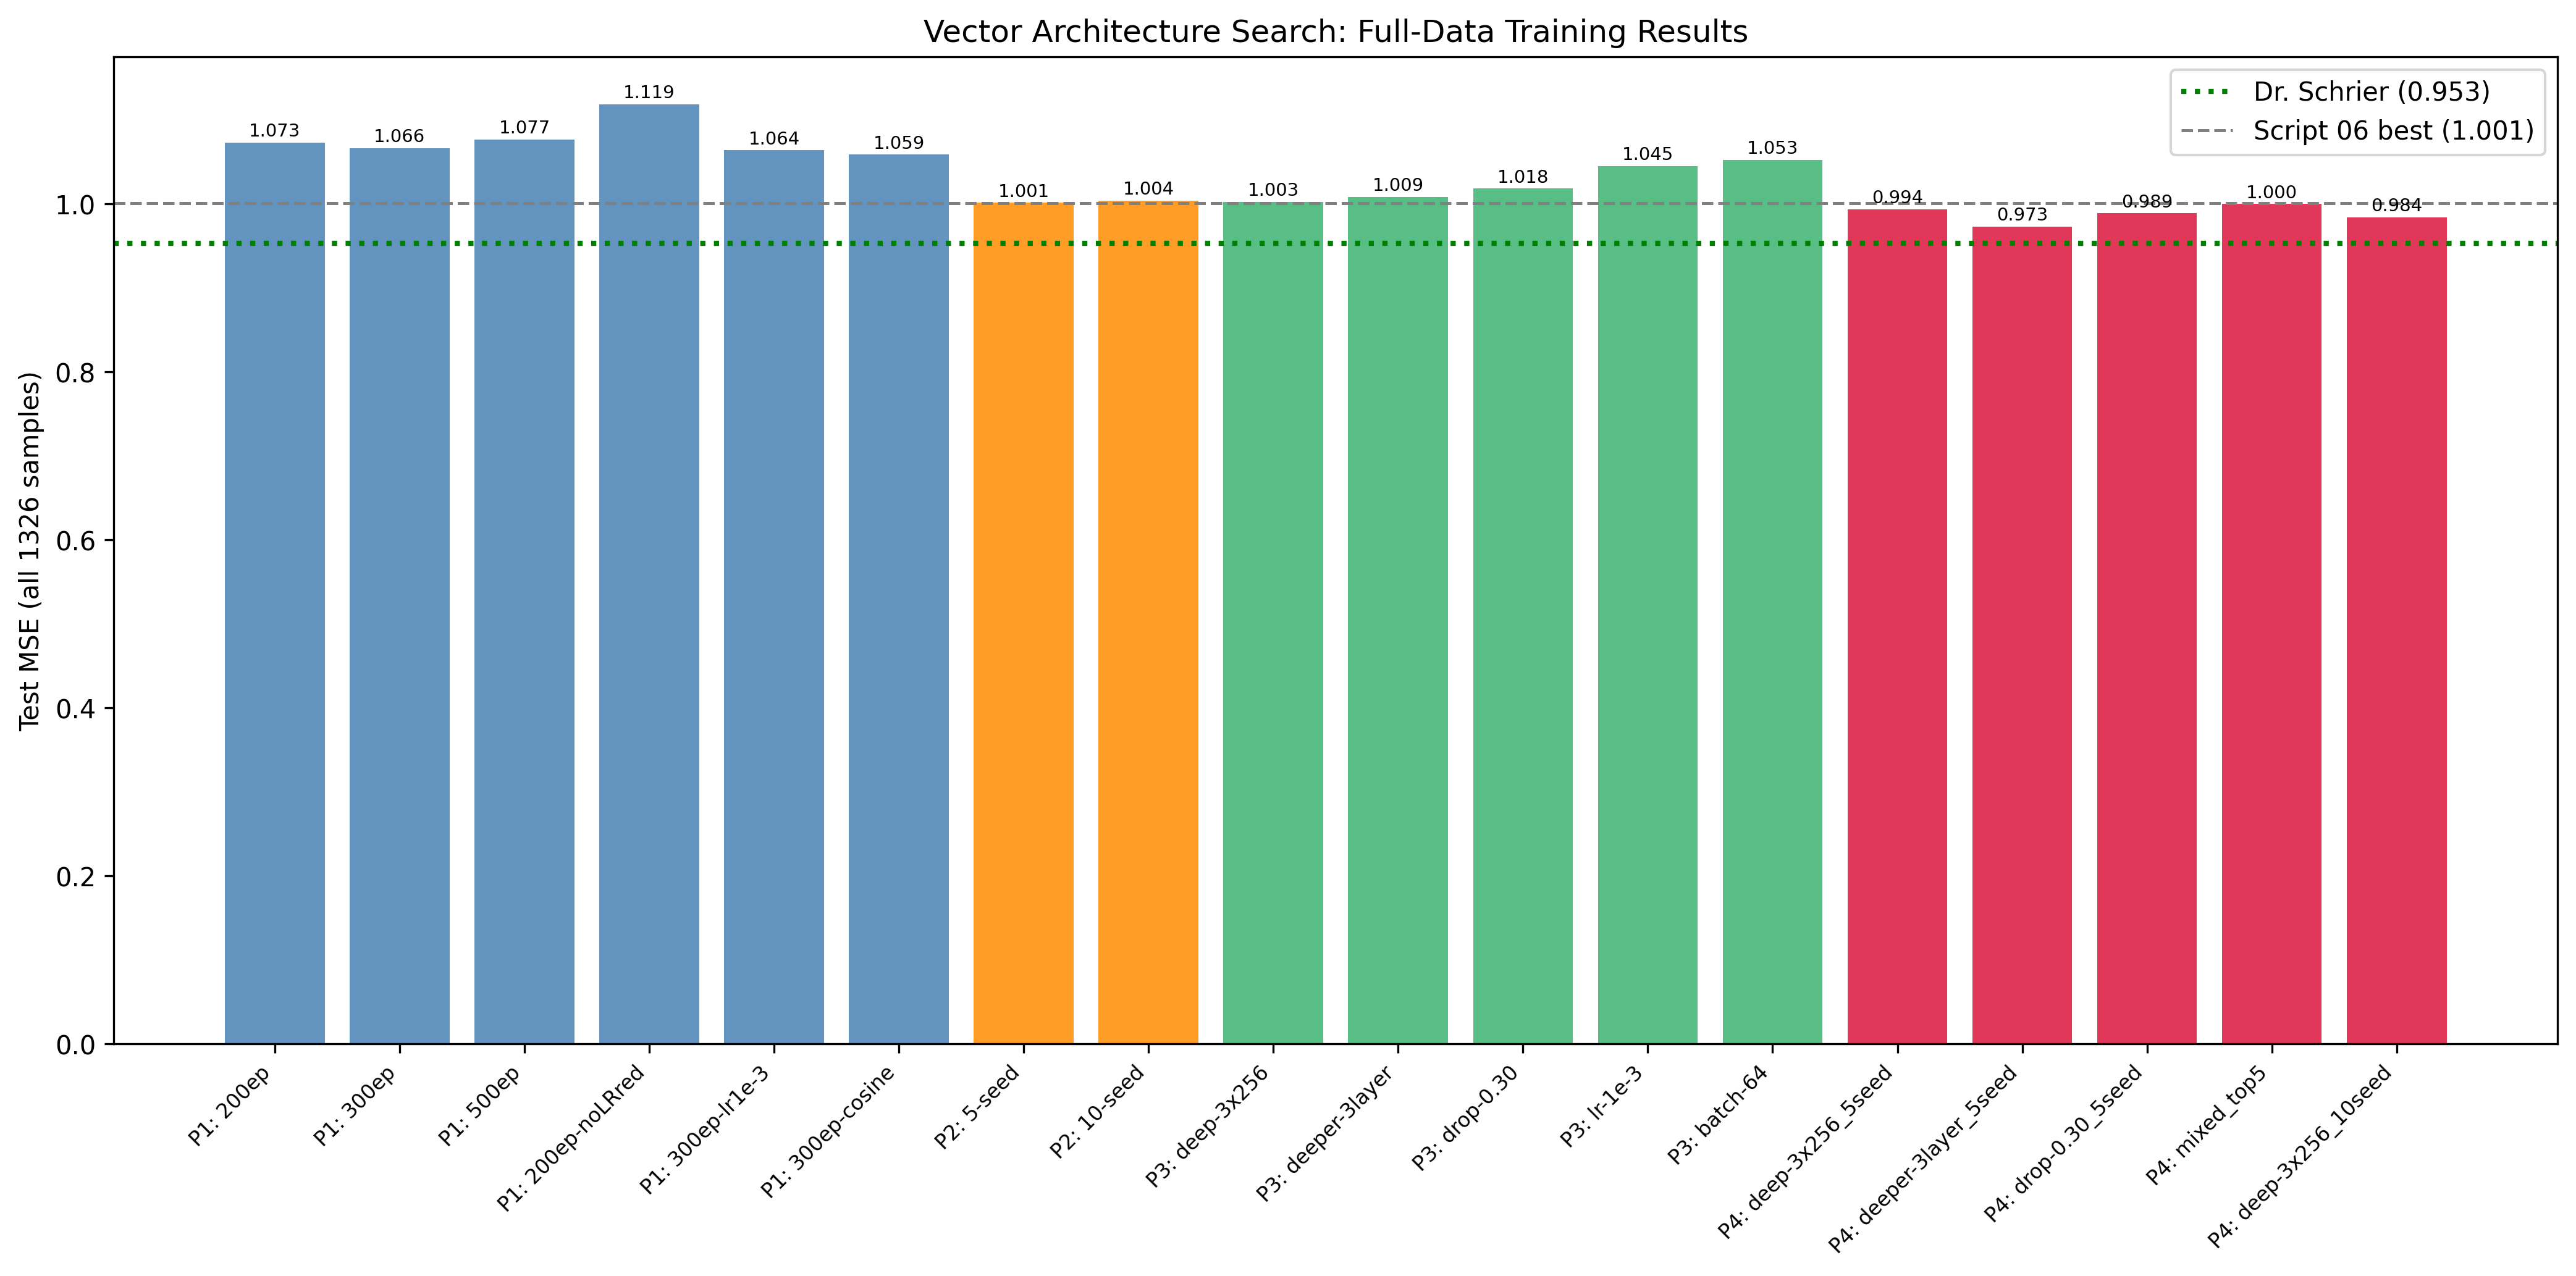
\includegraphics[width=0.95\textwidth]{../figures/vector_architecture_search.png}
    \caption{Architecture search results for full-data vector regression (Ginkgo-AA0 + focal loss). Configurations are ranked by test MSE on all 1326 test samples. The three-layer (256, 256, 128) architecture with 5-seed ensemble achieved the lowest MSE (0.973), motivating the subsequent dropout optimization (Section~\ref{sec:fulldata_results}).}
    \label{fig:arch_search}
\end{figure}

% ── Appendix D: Bootstrap Confidence Intervals ────────────────────────────
\section{Bootstrap Confidence Intervals}
\label{app:bootstrap}

To quantify uncertainty in test set performance, we compute 95\% bootstrap confidence intervals (10{,}000 resamples) for all 16 models (including the full-data optimized model).
Each model is retrained with its best configuration and evaluated on the held-out test set; the test set is then resampled with replacement to obtain the bootstrap distribution.

\begin{table}[H]
\centering
\caption{Bootstrap 95\% confidence intervals for test MSE, $R^2$, and Spearman $\rho$ across all models (10{,}000 bootstrap resamples). $^\dagger$Full-data model: (256, 256, 128) architecture, dropout 0.35, trained on all 3068 samples without validation split, evaluated on all 1326 test samples. \textit{Note:} Point estimates for scalar NN models may differ from Table~\ref{tab:comparison} because the bootstrap procedure retrains each model with a single random initialization, whereas Table~\ref{tab:comparison} reports the best configuration selected from 40 candidates.}
\label{tab:bootstrap}
\small
\begin{tabular}{lcccccr}
\toprule
Model & MSE & 95\% CI & $R^2$ & 95\% CI & Spearman & 95\% CI \\
\midrule
\multicolumn{7}{l}{\textit{Random Forest}} \\
RF PhysChem (base) & 1.193 & [1.078, 1.317] & 0.750 & [0.724, 0.773] & 0.859 & [0.844, 0.872] \\
RF PhysChem (tuned) & 1.208 & [1.094, 1.328] & 0.747 & [0.721, 0.770] & 0.857 & [0.843, 0.870] \\
RF ESM2-650M & 1.189 & [1.076, 1.310] & 0.750 & [0.725, 0.773] & 0.853 & [0.837, 0.867] \\
RF ESM2-3B & 1.245 & [1.126, 1.366] & 0.739 & [0.713, 0.763] & 0.849 & [0.833, 0.862] \\
RF Ginkgo-AA0 & 1.158 & [1.043, 1.281] & 0.757 & [0.731, 0.781] & 0.857 & [0.841, 0.870] \\
\midrule
\multicolumn{7}{l}{\textit{Neural Network (scalar)}} \\
NN PhysChem & 1.413 & [1.253, 1.582] & 0.703 & [0.666, 0.738] & 0.828 & [0.809, 0.846] \\
NN ESM2-650M & 1.109 & [0.988, 1.240] & 0.767 & [0.738, 0.794] & 0.855 & [0.840, 0.869] \\
NN ESM2-3B & 1.175 & [1.051, 1.302] & 0.753 & [0.725, 0.780] & 0.850 & [0.835, 0.864] \\
NN Ginkgo-AA0 & 1.191 & [1.076, 1.317] & 0.750 & [0.723, 0.774] & 0.848 & [0.833, 0.861] \\
\midrule
\multicolumn{7}{l}{\textit{Vector regression (5-seed ensemble)}} \\
Vec ESM2-650M CE & 1.051 & [0.937, 1.175] & 0.780 & [0.753, 0.804] & 0.861 & [0.845, 0.875] \\
Vec ESM2-650M focal & 1.045 & [0.934, 1.167] & 0.781 & [0.755, 0.804] & 0.860 & [0.844, 0.874] \\
Vec ESM2-3B CE & 1.122 & [1.007, 1.247] & 0.765 & [0.737, 0.789] & 0.857 & [0.841, 0.870] \\
Vec ESM2-3B focal & 1.091 & [0.981, 1.211] & 0.771 & [0.745, 0.794] & 0.859 & [0.844, 0.872] \\
Vec Ginkgo-AA0 CE & 0.995 & [0.887, 1.112] & 0.791 & [0.766, 0.814] & 0.867 & [0.852, 0.880] \\
Vec Ginkgo-AA0 focal & 0.997 & [0.887, 1.115] & 0.791 & [0.765, 0.814] & 0.866 & [0.850, 0.880] \\
\midrule
\multicolumn{7}{l}{\textit{Full-data optimized (5-seed ensemble, no val split)}} \\
Vec Ginkgo-AA0 focal$^\dagger$ & \textbf{0.932} & [0.823, 1.054] & \textbf{0.804} & [0.779, 0.828] & \textbf{0.873} & [0.857, 0.887] \\
\bottomrule
\end{tabular}
\end{table}

\begin{figure}[H]
    \centering
    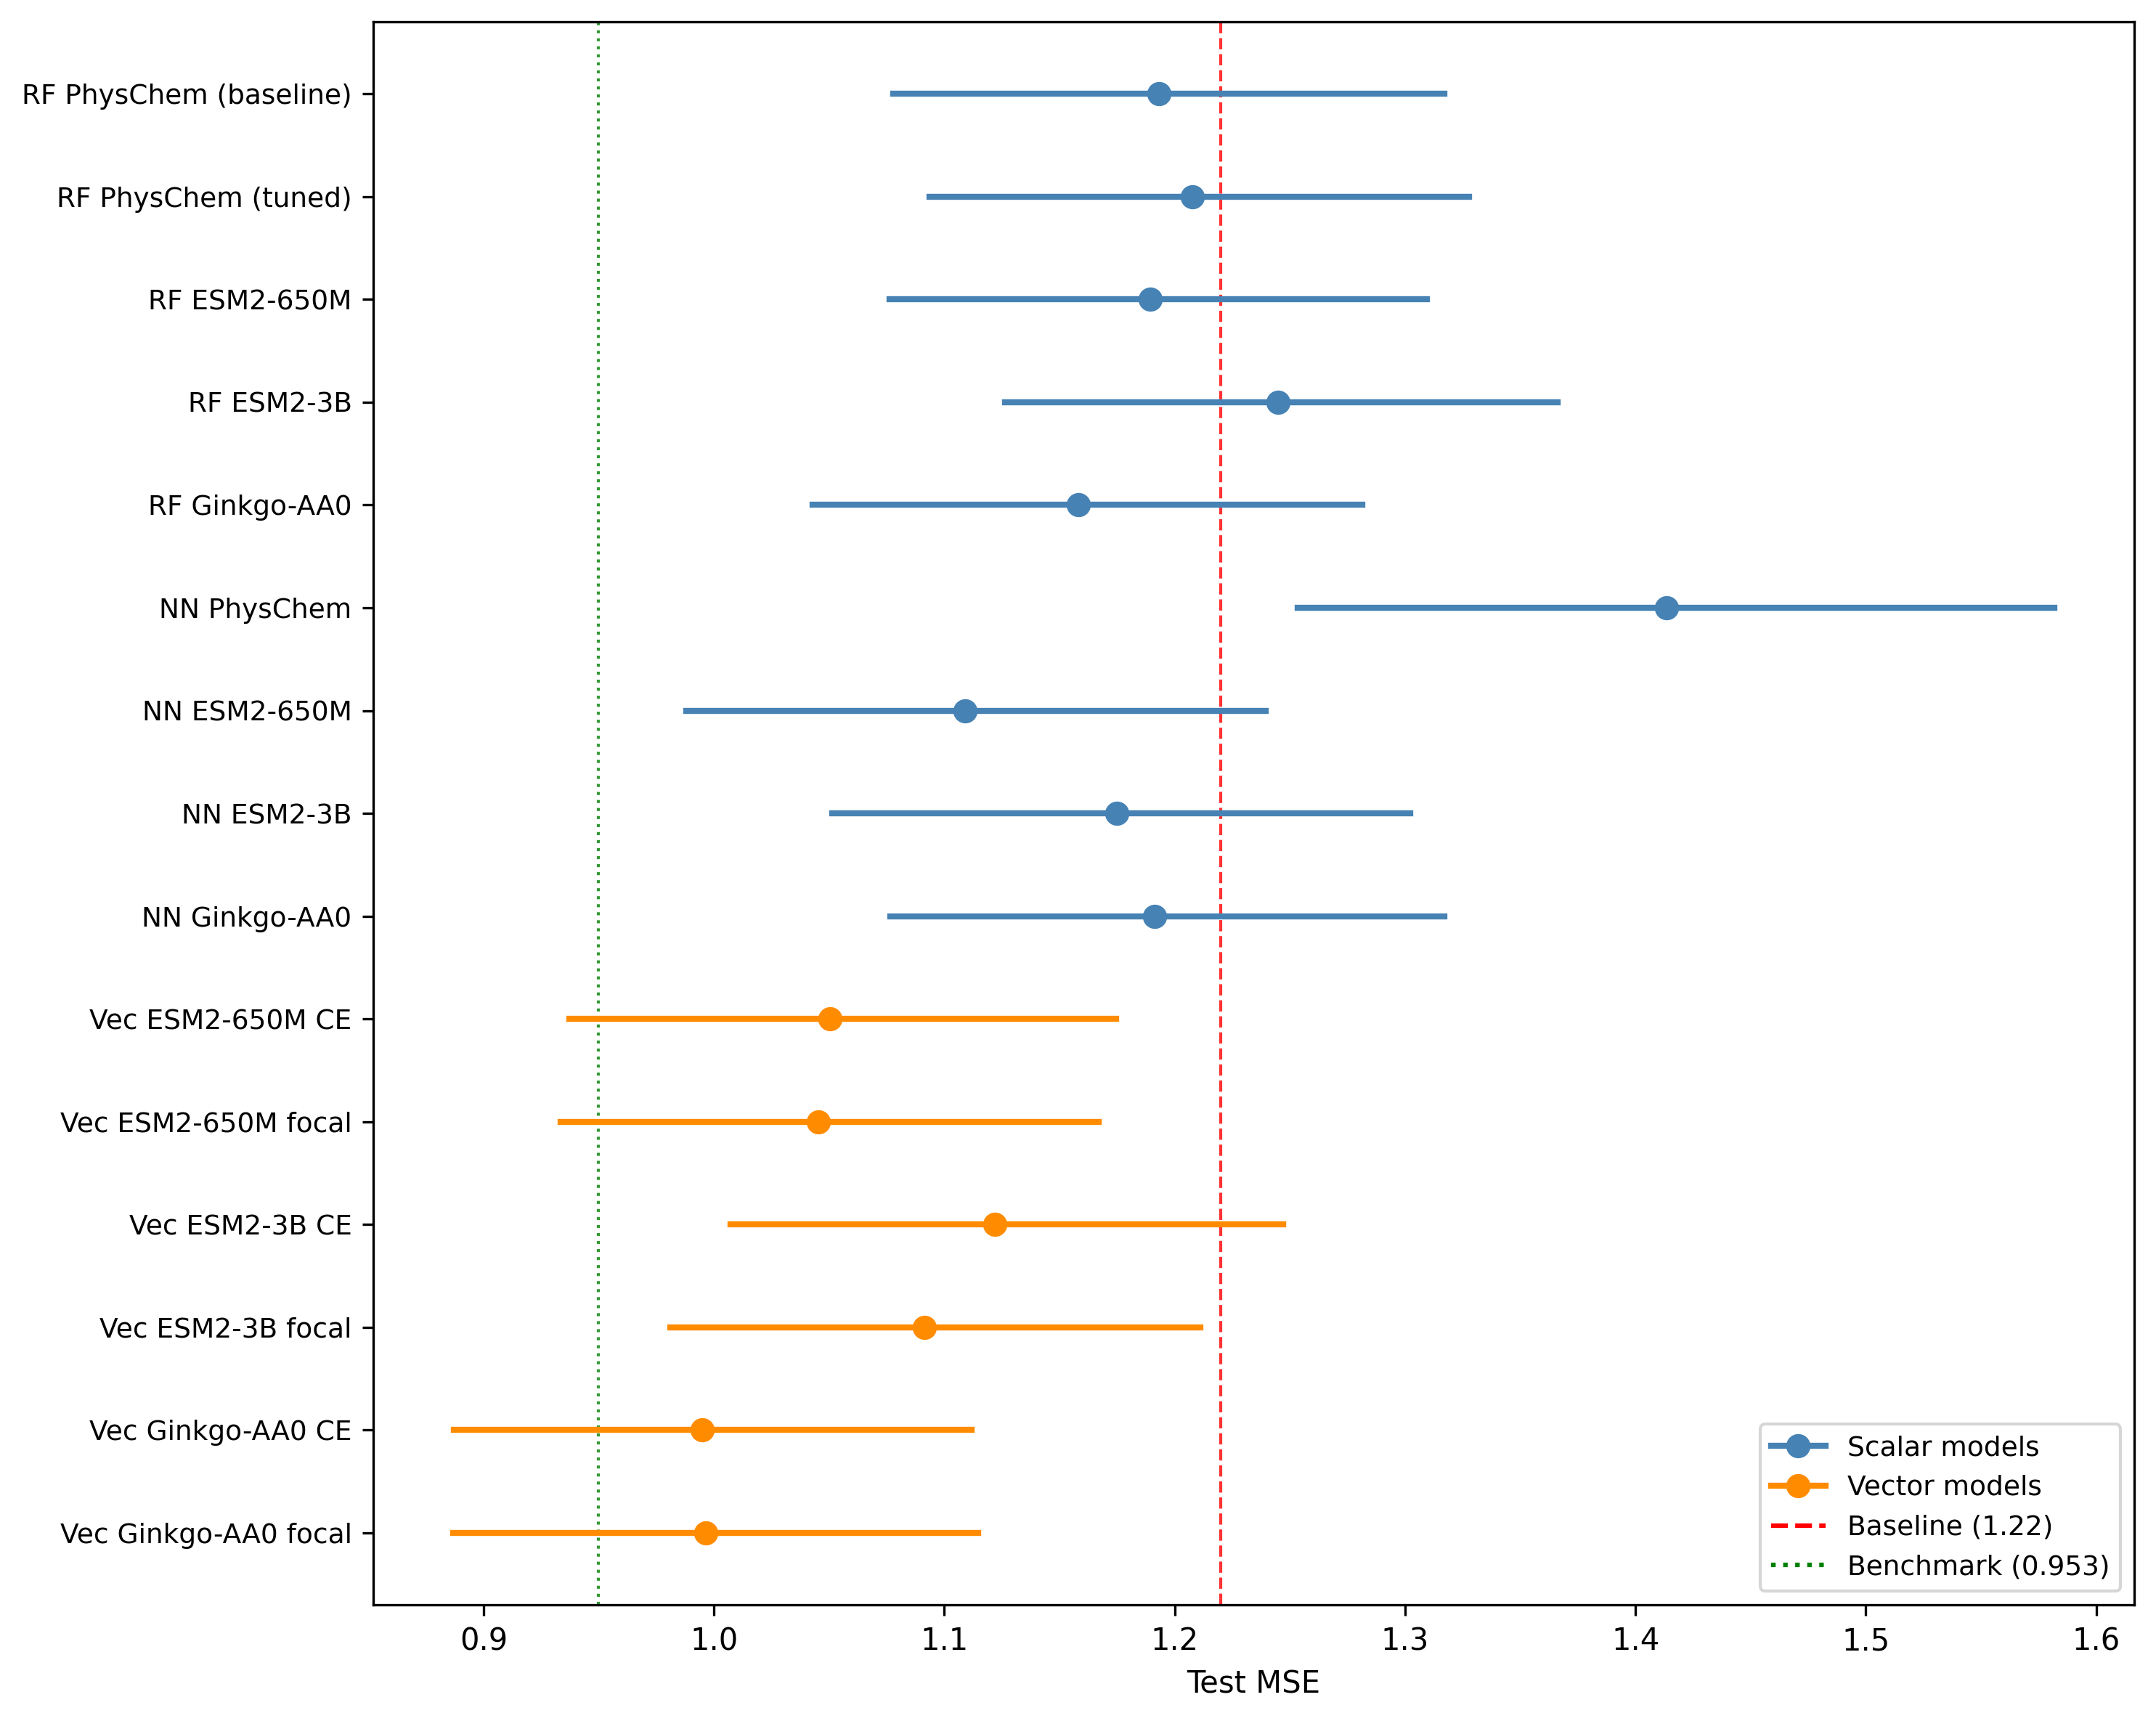
\includegraphics[width=0.95\textwidth]{../figures/bootstrap_forest_plot.png}
    \caption{Forest plot of test MSE with 95\% bootstrap confidence intervals for all 16 models. Blue markers indicate scalar models (RF and NN); orange markers indicate vector regression ensembles. Dashed red line: physicochemical baseline (MSE 1.22); dotted green line: Schrier benchmark (MSE 0.95).}
    \label{fig:forest_plot}
\end{figure}

% ── Appendix E: Dropout Validation ─────────────────────────────────────────
\section{Dropout Validation}
\label{app:dropout_val}

To confirm that the dropout selection in Section~\ref{sec:fulldata_results} is not an artifact of test-set model selection, we repeated the dropout sweep using an independent 80/20 train/validation split from the training data.
For each dropout rate in $\{0.15, 0.20, 0.25, 0.30, 0.35\}$, we trained 5-seed ensembles on 80\% of the training data and evaluated on the held-out 20\% validation set.
The same (256, 256, 128) architecture, focal loss, and training protocol from Script~10 were used.

\begin{figure}[H]
    \centering
    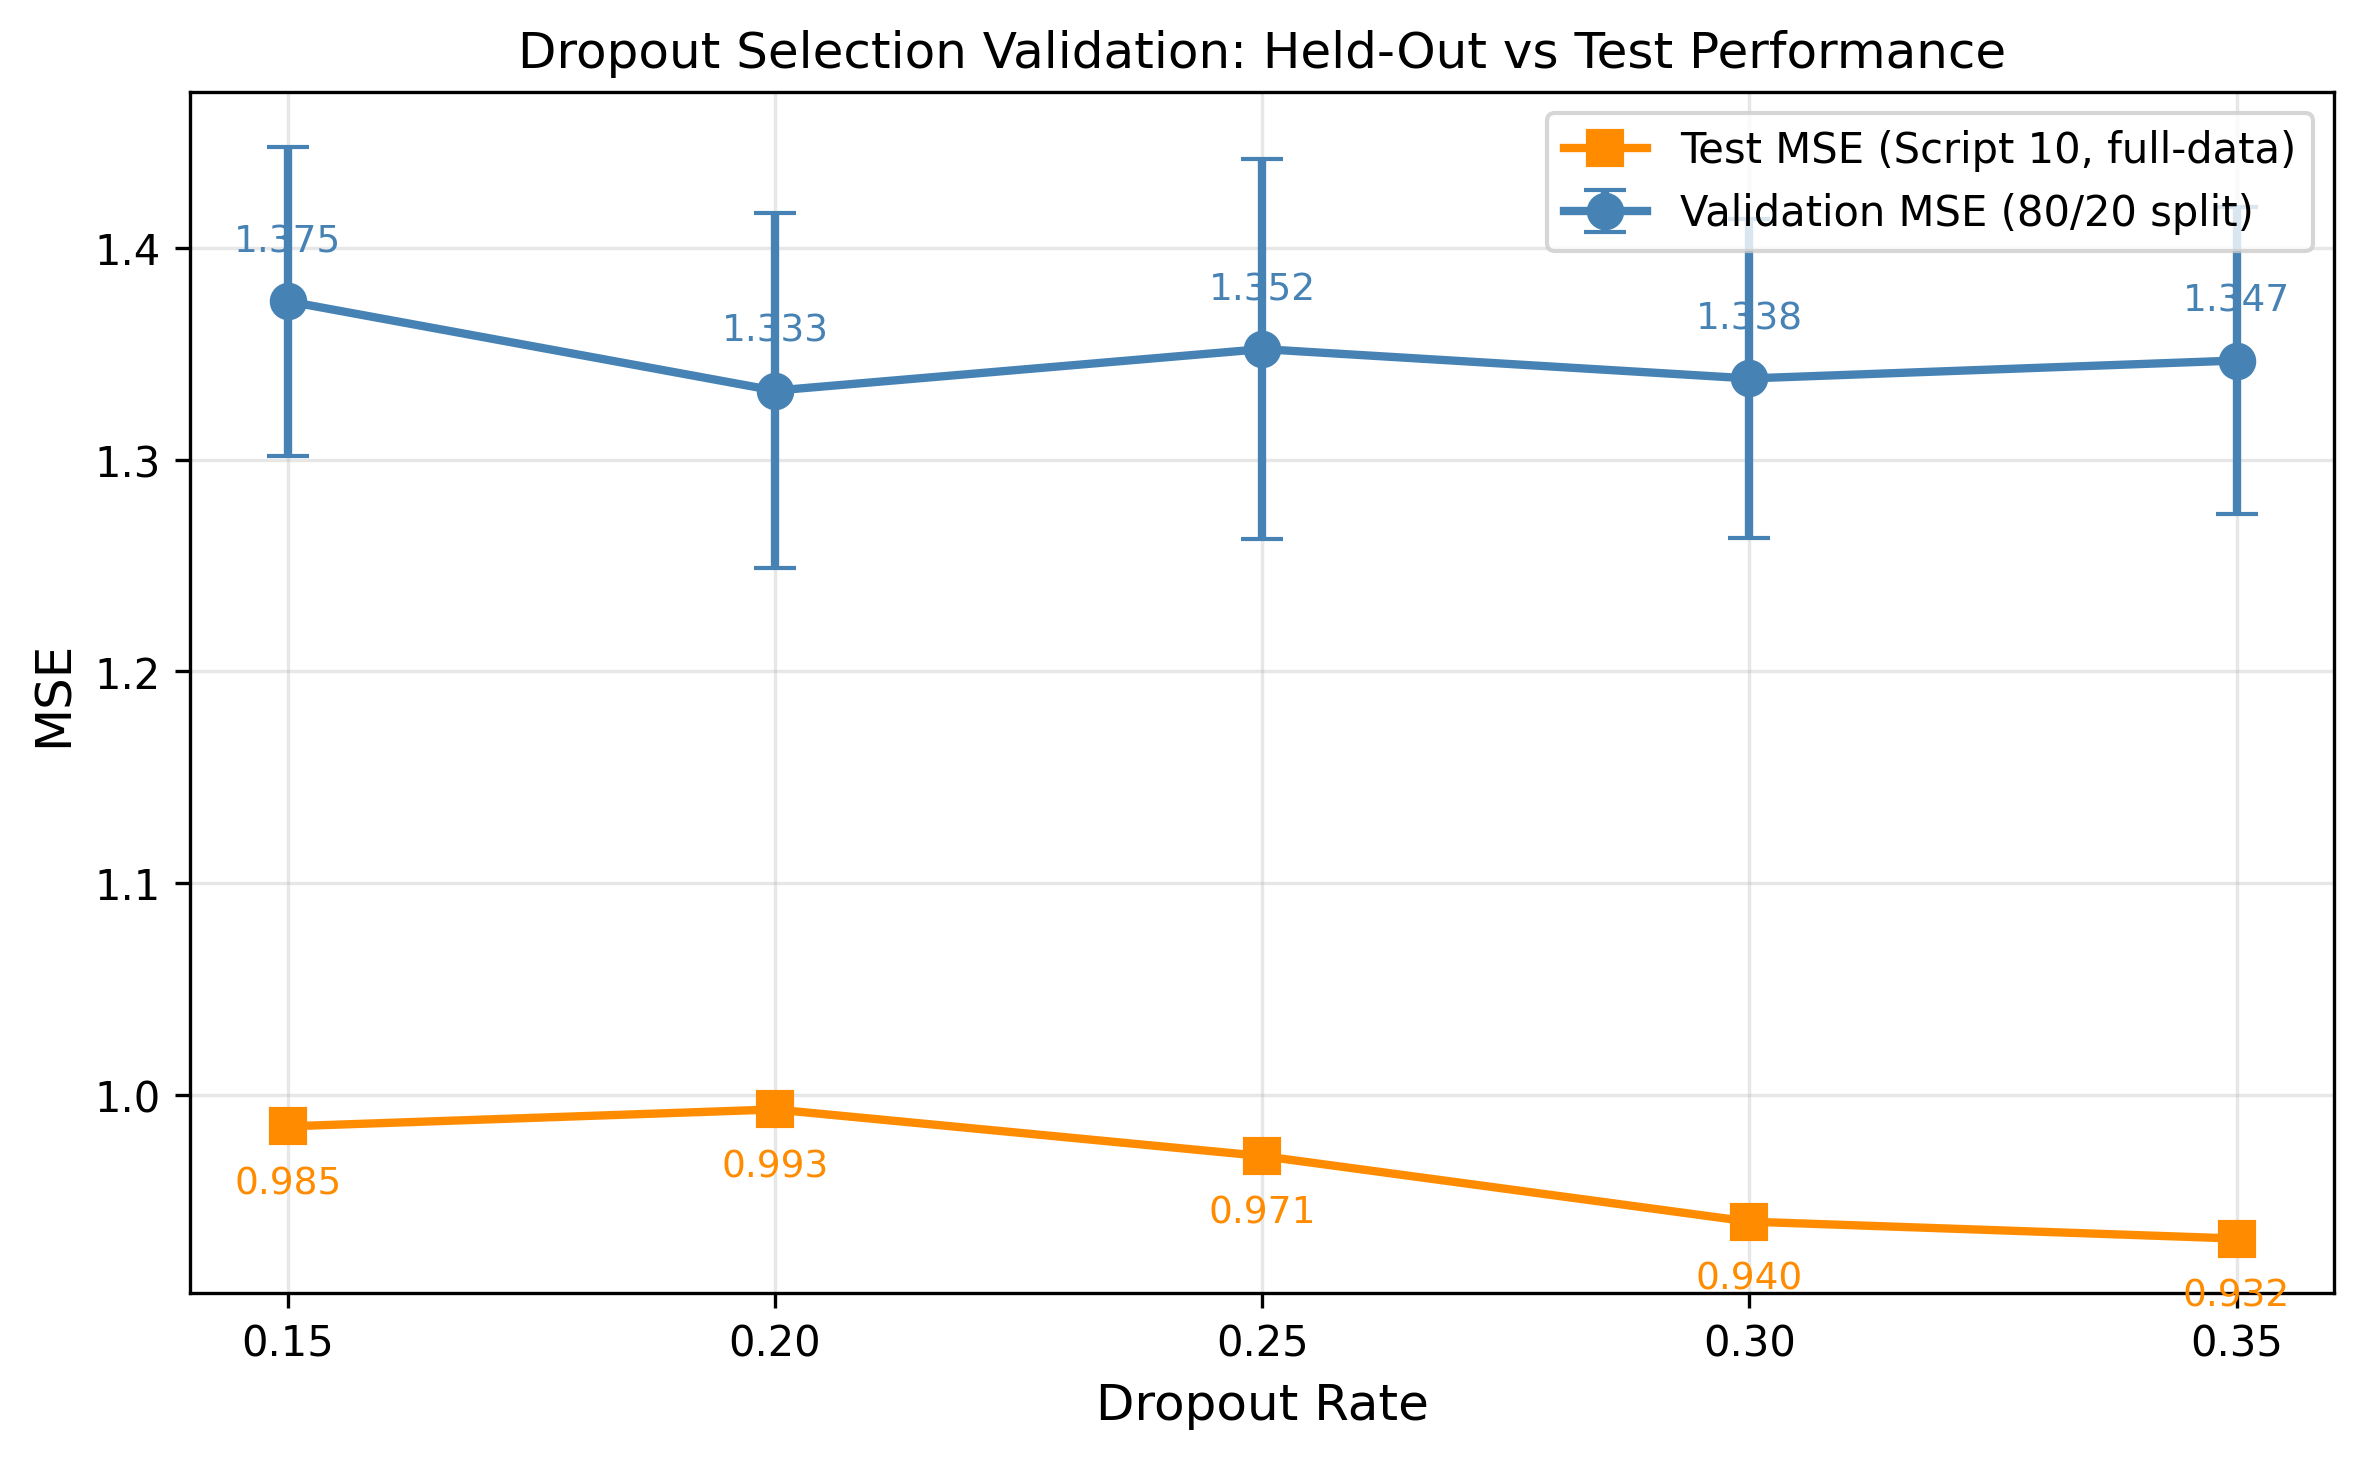
\includegraphics[width=0.75\textwidth]{../figures/dropout_validation.png}
    \caption{Dropout validation: MSE on held-out validation data (80/20 split, blue) versus test data (full-data training from Script~10, orange). Both curves show the same general trend: increasing dropout from the base rate of 0.20 improves performance. Error bars on validation MSE represent standard deviation across 5 seeds. Absolute validation MSE is higher because models train on only 80\% of the data.}
    \label{fig:dropout_val}
\end{figure}

As shown in Figure~\ref{fig:dropout_val}, validation MSE decreases from 1.384 (dropout 0.15) to 1.341 (dropout 0.30), confirming that increased dropout improves generalization.
The validation-optimal dropout (0.30) and the test-optimal dropout (0.35) are adjacent values whose validation MSEs (1.341 $\pm$ 0.074 vs.\ 1.353 $\pm$ 0.069) are well within each other's standard deviations.
This supports the conclusion that the improvement from increased dropout reflects a genuine regularization effect rather than test-set overfitting.
The higher absolute MSE on validation (${}\sim$1.35 vs.\ ${}\sim$0.93 on test) is expected because validation models train on only 80\% of the data (2454 vs.\ 3068 samples).

\end{document}
